% Blixem User Manual
% Author: Gemma Barson
%
% Run the following command twice to create a pdf of this manual
% (two runs are necessary to make sure all of the cross-references
% are up to date):
%
%    pdflatex Blixem_manual.tex
%
% This file was converted to LaTeX by Writer2LaTeX ver. 1.0.2
% see http://writer2latex.sourceforge.net for more info
%
\documentclass[letterpaper]{article}
\usepackage[latin1]{inputenc}
\usepackage[T1]{fontenc}
\usepackage[english]{babel}
\usepackage{amsmath}
\usepackage{amssymb,amsfonts,textcomp}
\usepackage{color}
\usepackage{array}
\usepackage{supertabular}
\usepackage{hhline}
\usepackage{hyperref}
\usepackage{titlesec}
\hypersetup{pdftex, colorlinks=true, linkcolor=blue, citecolor=blue, filecolor=blue, urlcolor=blue, pdftitle=Blixem User Manual, pdfauthor=Gemma Barson, pdfsubject=, pdfkeywords=}
\usepackage[pdftex]{graphicx}
% Paragraph styles
\setlength{\parindent}{0pt}
% Text styles
\newcommand\textstyleInternetlink[1]{\textcolor{blue}{#1}}
\newcommand\textstyleSourceText[1]{\texttt{#1}}
\newcommand\textstyleFootnoteSymbol[1]{\textsuperscript{#1}}
\definecolor{darkblue}{rgb}{0.2,0.3,0.5}
\definecolor{lightblue}{rgb}{0.3,0.5,0.8}
%\DeclareFixedFont{\sectionfont}{T1}{phv}{bx}{n}{16pt}
%\DeclareFixedFont{\subsectionfont}{T1}{phv}{bx}{n}{14pt}
%\DeclareFixedFont{\subsubsectionfont}{T1}{phv}{bx}{n}{12pt}
\titleformat{\section} {\normalfont\LARGE\bf\color{darkblue}}{\thesection}{1em}{}
\titleformat{\subsection} {\normalfont\large\bf\color{lightblue}}{\thesubsection}{1em}{}
\titleformat{\subsubsection} {\normalfont\normalsize\bf\color{lightblue}}{\thesubsubsection}{1em}{}
% Outline numbering
\setcounter{secnumdepth}{0}
\makeatletter
\newcommand\arraybslash{\let\\\@arraycr}
\makeatother
% List styles
\newcommand\liststyleLi{%
\renewcommand\labelitemi{{\textbullet}}
\renewcommand\labelitemii{{\textbullet}}
\renewcommand\labelitemiii{{\textbullet}}
\renewcommand\labelitemiv{{\textbullet}}
}
\newcommand\liststyleLii{%
\renewcommand\labelitemi{{\textbullet}}
\renewcommand\labelitemii{{\textbullet}}
\renewcommand\labelitemiii{{\textbullet}}
\renewcommand\labelitemiv{{\textbullet}}
}
\newcommand\liststyleLiii{%
\renewcommand\labelitemi{{\textbullet}}
\renewcommand\labelitemii{{\textbullet}}
\renewcommand\labelitemiii{{\textbullet}}
\renewcommand\labelitemiv{{\textbullet}}
}
\newcommand\liststyleWWviiiNumxxxvi{%
\renewcommand\labelitemi{{\textbullet}}
\renewcommand\labelitemii{o}
\renewcommand\labelitemiii{[F0A7?]}
\renewcommand\labelitemiv{[F0B7?]}
}
\newcommand\liststyleLiv{%
\renewcommand\labelitemi{{\textbullet}}
\renewcommand\labelitemii{${\circ}$}
\renewcommand\labelitemiii{${\blacksquare}$}
\renewcommand\labelitemiv{{\textbullet}}
}
\newcommand\liststyleWWviiiNumxxxi{%
\renewcommand\theenumi{\arabic{enumi}}
\renewcommand\theenumii{\alph{enumii}}
\renewcommand\theenumiii{\roman{enumiii}}
\renewcommand\theenumiv{\arabic{enumiv}}
\renewcommand\labelenumi{\theenumi.}
\renewcommand\labelenumii{\theenumii.}
\renewcommand\labelenumiii{\theenumiii.}
\renewcommand\labelenumiv{\theenumiv.}
}
\newcommand\liststyleWWviiiNumxxxv{%
\renewcommand\labelitemi{{\textbullet}}
\renewcommand\labelitemii{o}
\renewcommand\labelitemiii{[F0A7?]}
\renewcommand\labelitemiv{[F0B7?]}
}
\newcommand\liststyleWWviiiNumxiii{%
\renewcommand\labelitemi{{\textbullet}}
\renewcommand\labelitemii{o}
\renewcommand\labelitemiii{[F0A7?]}
\renewcommand\labelitemiv{[F0B7?]}
}
\newcommand\liststyleWWviiiNumxxvii{%
\renewcommand\labelitemi{{\textbullet}}
\renewcommand\labelitemii{o}
\renewcommand\labelitemiii{[F0A7?]}
\renewcommand\labelitemiv{[F0B7?]}
}
\newcommand\liststyleWWviiiNumxxvi{%
\renewcommand\labelitemi{{\textbullet}}
\renewcommand\labelitemii{o}
\renewcommand\labelitemiii{[F0A7?]}
\renewcommand\labelitemiv{[F0B7?]}
}
\newcommand\liststyleWWviiiNumxvi{%
\renewcommand\labelitemi{{\textbullet}}
\renewcommand\labelitemii{o}
\renewcommand\labelitemiii{[F0A7?]}
\renewcommand\labelitemiv{[F0B7?]}
}
\newcommand\liststyleWWviiiNumxxxvii{%
\renewcommand\labelitemi{{\textbullet}}
\renewcommand\labelitemii{o}
\renewcommand\labelitemiii{[F0A7?]}
\renewcommand\labelitemiv{[F0B7?]}
}
\newcommand\liststyleWWviiiNumxx{%
\renewcommand\labelitemi{{\textbullet}}
\renewcommand\labelitemii{o}
\renewcommand\labelitemiii{[F0A7?]}
\renewcommand\labelitemiv{[F0B7?]}
}
% Page layout (geometry)
\setlength\voffset{-1in}
\setlength\hoffset{-1in}
\setlength\topmargin{2.54cm}
\setlength\oddsidemargin{3.175cm}
\setlength\textheight{21.363003cm}
\setlength\textwidth{15.240001cm}
\setlength\footskip{1.497cm}
\setlength\headheight{0cm}
\setlength\headsep{0cm}
% Footnote rule
\setlength{\skip\footins}{0.119cm}
\renewcommand\footnoterule{\vspace*{-0.018cm}\setlength\leftskip{0pt}\setlength\rightskip{0pt plus 1fil}\noindent\textcolor{black}{\rule{0.25\columnwidth}{0.018cm}}\vspace*{0.101cm}}
% Pages styles
\makeatletter
\newcommand\ps@Standard{
  \renewcommand\@oddhead{}
  \renewcommand\@evenhead{}
  \renewcommand\@oddfoot{\thepage{}}
  \renewcommand\@evenfoot{\@oddfoot}
  \renewcommand\thepage{\arabic{page}}
}
\newcommand\ps@FirstPage{
  \renewcommand\@oddhead{}
  \renewcommand\@evenhead{}
  \renewcommand\@oddfoot{}
  \renewcommand\@evenfoot{}
  \renewcommand\thepage{\arabic{page}}
}
\makeatother
\pagestyle{Standard}
\setlength\tabcolsep{1mm}
\renewcommand\arraystretch{1.3}
% footnotes configuration
\makeatletter
\renewcommand\thefootnote{\arabic{footnote}}
\makeatother
\newcounter{Figure}
\renewcommand\theFigure{\arabic{Figure}}

\title{Blixem User Manual}
\author{Gemma Barson}
\date{2011-01-17}

\begin{document}

\setcounter{page}{1}\pagestyle{Standard}


\thispagestyle{FirstPage}
{\centering\sffamily\bfseries\color[rgb]{0.0,0.27058825,0.5254902}
\Huge\bf{Blixem User Manual}\par}

\bigskip

{\centering\large{Written by Gemma Barson}\par}
{\centering{\textless}\href{mailto:gb10@sanger.ac.uk}{gb10@sanger.ac.uk}{\textgreater}\par}

\bigskip

{\centering\large{Wellcome Trust Sanger Institute}\par}
{\centering17 January 2011\par}



\clearpage
{\color[rgb]{0.0,0.27058825,0.5254902}\section[Revision History]{Revision History}}
\hypertarget{RefHeading334316266717}{}

\begin{center}
\tablehead{}
\begin{supertabular}{|m{8.073cm}|m{3.2849998cm}|m{3.282cm}|}
\hline
\bfseries Revision &
\bfseries Date &
\bfseries Author\\\hline
 First revision (Blixem v4.1.5) &
 17/01/11 &
 Gemma Barson\\\hline
 Updated for Blixem v4.1.9 &
 14/02/11 &
 Gemma Barson\\\hline
 Updated for Blixem v4.1.13 &
 25/03/11 &
 Gemma Barson\\\hline
 Updated for Blixem v4.1.14 &
 05/04/11 &
 Gemma Barson\\\hline
 Updated for Blixem v4.1.17 &
 09/05/11 &
 Gemma Barson\\\hline
 Updated for Blixem v4.2 &
 17/06/11 &
 Gemma Barson\\\hline
 Updated for Blixem v4.7 &
 02/12/11 &
 Gemma Barson\\\hline
 Updated for Blixem v4.14 &
 15/06/12 &
 Gemma Barson\\\hline
 Updated for Blixem v4.26  &
 07/03/14 &
 Gemma Barson\\\hline
 &
 &
 \\\hline
 &
 &
 \\\hline
 &
 &
 \\\hline
 &
 &
 \\\hline
 &
 &
 \\\hline
 &
 &
 \\\hline
\end{supertabular}
\end{center}

\bigskip

\setcounter{tocdepth}{10}
\renewcommand\contentsname{Contents}

\clearpage\tableofcontents

\clearpage
{\color[rgb]{0.0,0.27058825,0.5254902}\section[Introduction]{Introduction}}
\hypertarget{RefHeading1421056909880}{}{
{This manual explains how to configure, run and
use Blixem. }{Blixem is an interactive
browser of pairwise matches displayed as multiple alignments. It is not
strictly a multiple alignment tool, rather a
{\textquotesingle}one-to-many{\textquotesingle} alignment. It is used
to check the alignments of nucleotide and amino acid sequences against
a reference sequence.}}


\bigskip

Blixem is maintained by the Wellcome Trust
Sanger Institute and is available as part of the SeqTools package.
The software can be downloaded from the Sanger
Institute{\textquoteright}s website:

\href{http://www.sanger.ac.uk/resources/software/seqtools/}
{\textstyleInternetlink{http://www.sanger.ac.uk/resources/software/seqtools}}

{\color[rgb]{0.30980393,0.5058824,0.7411765}\subsection[An aside about the name
{\textquotedblleft}Blixem{\textquotedblright}]{An aside about the name {\textquotedblleft}Blixem{\textquotedblright}}}
\hypertarget{RefHeading1441056909880}{}{
{{\textquotedblleft}BLIXEM{\textquotedbl} was
originally an acronym for
}{{\textquotedbl}BLast matches In an X-windows
Embedded Multiple alignment{\textquotedbl}, although this is a bit of a
misnomer now because Blixem can handle any kind of alignment, not just
BLAST matches. We have dropped the acronym, and the capital letters,
so the correct name is just
{\textquotedblleft}Blixem{\textquotedblright}.}}

\clearpage
{\color[rgb]{0.0,0.27058825,0.5254902}\section[Getting Started]{Getting Started}}
\hypertarget{RefHeading1461056909880}{}
{\color[rgb]{0.30980393,0.5058824,0.7411765}\subsection[Running Blixem]{Running Blixem}}
\hypertarget{RefHeading1481056909880}{}{
As a minimum, Blixem takes the following required arguments:}
\begin{quote}
\begin{verbatim}
blixem --display-type=N|P <features_file>
\end{verbatim}
\end{quote}
{where \texttt{{\textless}features\_file{\textgreater}} is the path name of a GFF
version 3 file containing the alignments and any other features. The
 \texttt{{\textquoteleft}{}-{}-display-type{\textquoteleft}} or
\texttt{{\textquoteleft}{}-t{\textquoteleft}} argument is the only mandatory
argument. It defines the display mode:
\texttt{{\textquoteleft}N{\textquoteleft}} for nucleotide or
\texttt{{\textquoteleft}P{\textquoteleft}} for protein. 
Run {\textquoteleft}blixem{\textquoteleft} without any arguments to see
further usage information.}

{\color[rgb]{0.30980393,0.5058824,0.7411765}\subsection[Input files]{Input files}}
\hypertarget{RefHeading1501056909880}{}{
Blixem takes one or two files as input: a mandatory GFF version 3 file
containing the features and, optionally, a separate file containing the
reference sequence in FASTA format.}

\bigskip

\begin{quote}
\begin{verbatim}
blixem --t N|P [<reference\sequence\file>] <features_file>
\end{verbatim}
\end{quote}

{If the reference sequence file is not provided, the reference sequence
must be supplied in FASTA format at the end of the GFF file, following
a comment line that reads {\textquoteleft}\#\#FASTA{\textquoteleft}.}


\bigskip

{\itshape
Note that the reference sequence must always be a nucleotide sequence
and match sequences must be the correct type for the mode, i.e.
nucleotide sequences for nucleotide mode or protein sequences for
protein mode.}

{\color[rgb]{0.30980393,0.5058824,0.7411765}\subsubsection[GFF file]{GFF file}}
\hypertarget{RefHeading1521056909880}{}{
Blixem uses the GFF version 3 file format. In this section we give a
very brief description of this file format; see
\url{http://www.sequenceontology.org/gff3.shtml} for a full
description.}

\bigskip

{The GFF file should start with the following two comment lines.
(Additional comments can be included but may be ignored.)

\bigskip

\begin{quote}
\begin{verbatim}
##gff-version 3
##sequence-region chr4-04 44144 154265
\end{verbatim}
\end{quote}
Each subsequent line defines a feature. A feature line must have the
following 8 tab-separated columns:
\begin{quote}
\begin{verbatim}
reference_sequence_name source type start end score strand phase}
\end{verbatim}
\end{quote}
An optional 9\textsuperscript{th} column defines any tags (separated by
semi-colons). Blixem supports the following GFF tags. (Additional
tags can be supplied but may be ignored.)}
\begin{center}
\begin{supertabular}{p{2.802cm}p{10.704cm}} 
\textbf{Target } & (required for alignments) \\
\textbf{Gap}  & (required for gapped alignments) \\
\textbf{ID } & (required for parent features) \\
\textbf{Name } & (required for transcripts and SNPs) \\
\textbf{Parent } & (required for child features) \\
\end{supertabular}
\end{center}

{In addition, Blixem supports the following custom tags.}
\begin{center}
\begin{supertabular}{p{2.802cm}p{10.704cm}} 
\textbf{percentId} & (only applicable to alignments; populates the \%ID column) \\
\textbf{sequence } & (only applicable to alignments; supplies thesequence data) \\
\textbf{variant\_sequence} & (only applicable to variations; supplies the variation data) \\
\textbf{url } & (only used by variations; GFF3 special characters must be escaped) \\
\end{supertabular}
\end{center}

{\color[rgb]{0.30980393,0.5058824,0.7411765}\subsubsection[Transcripts]{Transcripts}}

{Note that exons should have a Parent transcript defined, and the Name
tag should be set in the parent rather than the child exons. Note
that Blixem \textit{will} recognise exons that do not have a Parent tag
if they have a Name tag instead, but they may not get grouped correctly
with other exons from the same transcript.}

\bigskip

{Typically, one defines the parent transcript, the exons, and the CDS
regions; Blixem will then calculate the missing components (in this
case, the UTR regions and the introns). Blixem will recognise other
combinations of inputs, and will always calculate the missing
components as long as enough information is provided. }

\bigskip

{\color[rgb]{0.30980393,0.5058824,0.7411765}\subsubsection[Variations]{Variations}}

{SNPs, insertions and deletions are supported, as well as combined
variations. One may use the generic
{\textquoteleft}sequence\_alteration{\textquoteleft} type for these but
it is good practice to use more specific types such as
{\textquoteleft}SNP{\textquoteleft} or
{\textquoteleft}deletion{\textquoteleft} where applicable.}

\bigskip

{\color[rgb]{0.30980393,0.5058824,0.7411765}\subsubsection[Sample GFF file]{Sample GFF file}}

{A sample GFF file may look like this
({\textquoteleft}{\dots}{\textquoteleft} denotes that text has been
omitted).}

\bigskip

\begin{quote}
\begin{verbatim}
##gff-version 3
##sequence-region chr4-04 44144 154265
chr4-04 EST_Human nucleotide_match 79195 79311 95.000000 - . Target=DA692754\
.1 287 403 +;percentID=90.6;sequence=GATCTGGC...
chr4-04 EST_Human nucleotide_match 79195 79323 121.000000 + . Target=AI09510\
3.1 326 454 +;percentID=96.9;sequence=TTTAAATT...
chr4-04 ensembl_variation deletion 80798 80799 . + . Name=rs60725655;url=htt\
p%3A%2F%2Fwww.ensembl.org%2FHomo_sapiens%2FVariation%2FSummary%3Fv%3Drs60725\
655;variant_sequence=AA/-;
chr4-04 ensembl_variation sequence_alteration 80799 80799 . + . Name=rs57681\
246;url=http%3A%2F%2Fwww.ensembl.org%2FHomo_sapiens%2FVariation%2FSummary%3F\
v%3Drs57681246;variant_sequence=A/-/C;
chr4-04 ensembl_variation SNP 81040 81040 . + . Name=rs2352935;url=http%3A%2\
F%2Fwww.ensembl.org%2FHomo_sapiens%2FVariation%2FSummary%3Fv%3Drs2352935;var\
iant_sequence=T/C;
chr4-04 ensembl_variation insertion 82229 82230 . + . Name=rs35105663;url=ht\
tp%3A%2F%2Fwww.ensembl.org%2FHomo_sapiens%2FVariation%2FSummary%3Fv%3Drs3510\
5663;variant_sequence=-/G;
chr4-04 Augustus mRNA 119534 119941 . - . ID=transcript21;Name=AUGUSTUS00000\
051712
chr4-04 Augustus exon 119534 119941 . - . Parent=transcript21
chr4-04 Augustus CDS 119534 119941 . - 0 Parent=transcript21
\end{verbatim}
\end{quote}

\bigskip

{\color[rgb]{0.30980393,0.5058824,0.7411765}\subsubsection[FASTA file]{FASTA file}}
\hypertarget{RefHeading1541056909880}{}{
A FASTA file has a header line that starts with
{\textquoteleft}{\textgreater}{\textquoteright}. We use a custom
FASTA header format that contains the sequence name followed by the
start and end coordinates, separated by spaces. Note that the FASTA
sequence range may be different to the GFF file range.}

{The next line contains the start of the sequence data. The sequence
data can be on a single line or separated by newlines; it is usually
separated by newlines every 50 characters to aid readability.}

\bigskip

\begin{quote}
\begin{verbatim}
>chr4-04 44144 154265
tcttgtttctgtaggagaggccatctccatcagctataaccaaaaaaaaa
acaaaaaactcctctttttgacaagtttgtaaagcctgtccatctgggtc
tataataatcctccaggccctatgccactcctctttattcagccagttca
...
\end{verbatim}
\end{quote}

{\color[rgb]{0.30980393,0.5058824,0.7411765}\subsubsection[Combined GFF and FASTA file]{Combined GFF and FASTA file}}

\begin{quote}
\begin{verbatim}
##gff-version 3
##sequence-region chr4-04 44144 154265
chr4-04_210623-364887 EST_Human nucleotide_match 79195 79311 95.000000 - . \
Target=DA692754.1 287 403 +;percentID=90.6
chr4-04_210623-364887 EST_Human nucleotide_match 79195 79323 121.000000 + .\
 Target=AI095103.1 326 454 +;percentID=96.9
...
##FASTA
>chr4-04 44144 154265
tcttgtttctgtaggagaggccatctccatcagctataaccaaaaaaaaa
acaaaaaactcctctttttgacaagtttgtaaagcctgtccatctgggtc
tataataatcctccaggccctatgccactcctctttattcagccagttca
...
\end{verbatim}
\end{quote}

{\color[rgb]{0.30980393,0.5058824,0.7411765}\subsection[Configuration file]{Configuration file}}
{Blixem supports {\textquotedblleft}.ini-style{\textquotedblright}
configuration files which are used to specify user options and to tell
Blixem how to handle particular types of data. Blixem can accept
config files by one or both of the following methods:}

\liststyleLi
\begin{itemize}
\item {
A default config file called \textstyleSourceText{\textrm{.blixemrc}}
located in the user{\textquotesingle}s home directory. }
\item {
A file passed on the command-line using the
\textstyleSourceText{\textrm{{}-c}} argument. The contents of this file
will take priority if there are any clashes with the default file. }
\end{itemize}

{The default config file is generally used for display settings that are
set from the Settings dialog. Blixem saves display settings to this
file on exit, so it will be created the first time Blixem exits if it
does not already exist. You can also edit this file by hand or add
system settings to it such as the fetch methods if you wish. }

\bigskip

{The command-line method is useful when Blixem is called as part of a
pipeline, because it allows the calling program to set specific config
options (commonly the data-handling properties). }

{\color[rgb]{0.30980393,0.5058824,0.7411765}\subsubsection[Program defaults]{Program defaults}}
\hypertarget{RefHeading37691724351149}{}{
Defaults for the program can be specified in the
\textstyleSourceText{\textrm{[blixem]}} stanza. The properties that can
be set are described below. }

\bigskip

\begin{quote}
\begin{verbatim}
[blixem]
link-features-by-name=false
squash-linked-features=true
squash-identical-features=false
bulk-fetch = none
user-fetch = internal
stylesfile = ~/.ZMap/styles.ini
\end{verbatim}
\end{quote}

{\textstyleSourceText{\textrm{\textbf{link-features-by-name}}}\textbf{ }}

{If true, features with the same name are considered to have the same
parent, e.g. exons and introns with the same name are part of the same
transcript, or matches with the same name are from the same match
sequence. }

\bigskip

{\textstyleSourceText{\textrm{\textbf{squash-linked-features}}}\textbf{ }}

{If true, features that are linked under the same parent are squashed onto the same line when 'squash matches' is on.}

\bigskip

{\textstyleSourceText{\textrm{\textbf{squash-identical-features}}}\textbf{ }}

{If true, matches that are identical are squashed onto the same line when 'squash matches' is on.}

\bigskip

{\textstyleSourceText{\textrm{\textbf{bulk-fetch}}}\textbf{ }}

{This specifies the default method to use when batch-fetching sequences
on start-up. Its value must be one of the fetch methods specified in
the fetch method stanzas. The results of the fetch are parsed by
Blixem. The bulk-fetch method can be overriden for specific data types
(see the Data types section). }

\bigskip

{A comma-separated list of fetch methods can be specified if alternative
fetch methods should be used if the first fetch fails for some reason.
Each fetch method is tried in turn, in the order listed, until all
sequences have been successfully fetched or we run out of methods to
try.}

\bigskip

{\textstyleSourceText{\textrm{\textbf{user-fetch}}}\textbf{ }}

{This specifies the default method to use when the user interactively
fetches a sequence from within Blixem, i.e. by double-clicking on a
sequence. Its value must be one of the fetch methods specified in the
fetch method stanzas. The results of the fetch are displayed to the
user. The user-fetch method can be overridden for specific data types
(see the Data types section). }

\bigskip

{A comma-separated list of fetch methods can be specified if alternative
fetch methods should be used if the first fetch fails for some reason.
Each fetch method is tried in turn, in the order listed, until the
sequence has been successfully fetched or we run out of methods to try.}

\bigskip

{\textstyleSourceText{\textrm{\textbf{stylesfile}}}\textbf{ }}

This specifies an ini-type file which is used to specify the colours that should be used for features in Blixem's transcript view. The file should contain one or more source stanzas followed by one or more key=value pairs, i.e.

\begin{quote}
\begin{verbatim}
[<source>]
<key>=<value>
...
\end{verbatim}
\end{quote}

\texttt{{\textless}key{\textgreater}} can be one of:
\begin{quote}
\texttt{colours}: default colours

\texttt{transcript-cds-colours}: used to specify a different colour for CDS sections
\end{quote}

\bigskip

\texttt{{\textless}value{\textgreater}} is a semi-colon separated list of fill and line colours of the format

\begin{quote}
\begin{verbatim}
<normal|selected> <fill|border> <colour>
\end{verbatim}
\end{quote}

\texttt{{\textless}colour{\textgreater}} can be in any of the forms accepted by XParseColor; these include name for a colour from rgb.txt, such as DarkSlateGray, or a hex specification such as \texttt{\#305050}.

\bigskip

{\textstyleSourceText{\textrm{\textbf{Example}}}\textbf{}}
\begin{quote}
\begin{verbatim}
colours=normal border #0000af ; selected border #0000af ; normal fill white ;\
selected fill #ffddcc ; 
transcript-cds-colours=normal border #0000af ; selected border #0000af ; norm\
al fill white ; selected fill #ffddcc ;
\end{verbatim}
\end{quote}

Note that selection colors will be calculated automatically if they are not specified (a darker shade of the default color will be used when the feature is selected).

{\color[rgb]{0.30980393,0.5058824,0.7411765}\subsubsection[Fetch methods ]{Fetch methods }}
{These stanzas define custom methods for fetching sequence data. Each
fetch method must specify the \textstyleSourceText{fetch-mode} key,
which determines what type of fetch to perform. Other keys depend on
the fetch mode. Valid fetch modes and their required keys are: }

\liststyleLii
\begin{itemize}
\item {\ttfamily\textbf{socket}: node, port, command, args }
\item {\ttfamily\textbf{http}: url, port, cookie-jar, request }
\item {\ttfamily\textbf{command}: command, args }
\item {\ttfamily\textbf{sqlite}: location, query }
\item {\ttfamily\textbf{www}: url, request (user-fetch only; opens browser) }
\item {\ttfamily\textbf{internal}: (user-fetch only; displays stored sequence) }
\item {\ttfamily\textbf{none}: none }
\end{itemize}

\bigskip

{
In addition, the following keywords are required for bulk-fetch methods:
}

\liststyleLii
\begin{itemize}
\item {\texttt{\textbf{separator}}: Specifies the separator between multiple sequence names when they are compiled into a list. }
\item {
\texttt{\textbf{output}}: Defines the output format and can be one of the following: 
\begin{itemize}
\item {\texttt{raw}: raw sequence data; each sequence separated by a new line}
\item {\texttt{fasta}: FASTA format }
\item {\texttt{embl}: EMBL format }
\item {\texttt{list}: A list of named columns is returned }
\item {\texttt{gff}: GFF format for re-parsing }
\end{itemize}}
\end{itemize}

\bigskip

{
The following optional keywords can also be included for any fetch
method: }

\liststyleLii
\begin{itemize}
\item {
\texttt{\textbf{errors}}: Specifies a list of known error messages. This
is used by Blixem to determine whether an error occurred even if the
fetch program executed successfully. The value should be a
comma-separated list of the expected error message text, e.g.
\textstyleSourceText{error={\textquotedbl}no
match{\textquotedbl},{\textquotedbl}Not
authorized{\textquotedbl}}\texttt{ }}
\end{itemize}

\bigskip

{
The \textstyleSourceText{request} and
\textstyleSourceText{\textrm{args}} values can include the following
substitution symbols, which will be populated by blixem at run time.
Use \texttt{\%\%} to represent a normal \texttt{\%} character. }

\liststyleLii
\begin{itemize}
\item {
\texttt{\textbf{\%p}}: program name }
\end{itemize}
\liststyleLii
\begin{itemize}
\item {\texttt{\textbf{\%h}}: host name }
\item {\texttt{\textbf{\%u}}: user name }
\item {\texttt{\textbf{\%m}}: match sequence name(s) }
\item {\texttt{\textbf{\%r}}: reference sequence name }
\item {\texttt{\textbf{\%s}}: start coord of feature on reference sequence }
\item {\texttt{\textbf{\%e}}: end coord of feature on reference sequence }
\item {\texttt{\textbf{\%d}}: dataset }
\item {\texttt{\textbf{\%S}}: feature source }
\item {\texttt{\textbf{\%f}}: file name (specified in the file tag in the GFF or in the Source stanza) }
\item {\texttt{\textbf{\%(<key>)}}: where \texttt{<key>} is any named key in the Source stanza }


\bigskip
\end{itemize}

\begin{quote}
\begin{verbatim}
[pfetch-socket]
fetch-mode=socket
node=pfetch.sanger.ac.uk
port=22400
command=pfetch
args=--client=%p_%h_%u -q -C -F %m
errors="no match"","Not authorized"
separator=" "
output=embl

[pfetch-http]
fetch-mode=http
url=http://www.sanger.ac.uk:80/cgi-bin/otter/65/pfetch
request=request=%m
port=80}
cookie-jar=/nfs/users/nfs_g/gb10/.otter/ns_cookie_jar
errors="no match","Not authorized"
separator=" "
output=fasta

[www-fetch]
fetch-mode=www
url=http://www.sanger.ac.uk/cgi-bin/otter/65/pfetch
request=request=-F \%m

[variation-fetch]
fetch-mode=www
url=http://www.ensembl.org/Homo_sapiens/Variation/Summary
request=v=%m

[bam-fetch]
fetch-mode=command
command=bam_get
args=-file=http://hgdownload-test.cse.ucsc.edu/goldenPath/hg19/encodeDCC/wgEncode\
CshlLongRnaSeq/releaseLatest/%f
-chr_prefix=chr -gff_feature_source=%S -chr=%r -start=%s -end=%e
-dataset=%d
output=gff

[internal]
fetch-mode=internal

[none]
fetch-mode=none
\end{verbatim}
\end{quote}

{\color[rgb]{0.30980393,0.5058824,0.7411765}\subsubsection[Data types ]{Data types }}
\hypertarget{RefHeading37731724351149}{}{
You can override Blixem defaults by specifying a data-type for specific
features. Data-types can be specified by a source mapping using the
\texttt{[source-data-types]} stanza, or by using the custom
\textstyleSourceText{dataType} tag in the GFF input file. Possible
key-value pairs are the same as for the Program defaults. }

\bigskip

\begin{quote}
\begin{verbatim}
[dna-match]
link-features-by-name=true
bulk-fetch=pfetch-socket-embl,pfetch-socket-fasta
user-fetch=pfetch-http-embl,pfetch-http-fasta,internal

[protein-match]
link-features-by-name=true
bulk-fetch=pfetch-socket-fasta
user-fetch=pfetch-socket-embl,pfetch-socket-fasta,internal

[ensembl-variation]
user-fetch=variation-fetch
\end{verbatim}
\end{quote}

{\color[rgb]{0.30980393,0.5058824,0.7411765}\subsubsection[Source mapping ]{Source mapping }}
\hypertarget{RefHeading37751724351149}{}{
This stanza allows you to map a source to a particular data type. The
keys should be valid sources that appear in the GFF file ,and the
values must be stanzas specified in the data-type stanzas. }

\bigskip

\begin{quote}
\begin{verbatim}
[source-data-types]
EST_Human=dna-match
EST_Mouse=dna-match
EST_Pig=dna-match
EST_Other=dna-match
SwissProt=protein-match
TrEMBL=protein-match
ensembl_variation=ensembl-variation
\end{verbatim}
\end{quote}

{\color[rgb]{0.30980393,0.5058824,0.7411765}\subsubsection[Sources ]{Sources }}
\hypertarget{RefHeading37771724351149}{}
These stanzas allow you to set additional information on a per-source basis. You can substitute any value specified here using the \texttt{\%(<key>)} substitution format, e.g. in the following example you could include the filename by using the substitution variable \texttt{\%(file)}.

\bigskip

\begin{quote}
\begin{verbatim}
[Tier2_HepG2_cytosol_longPolyA_rep2]
file=wgEncodeCshlLongRnaSeqHepg2CytosolPapAlnRep2.bam
\end{verbatim}
\end{quote}

{\color[rgb]{0.30980393,0.5058824,0.7411765}\subsubsection[User settings ]{User settings }}
\hypertarget{RefHeading37791724351149}{}{
The following stanzas are used to specify display settings via the
config file, that is, settings that the user can change via the
Settings dialog in Blixem. These are saved to the default config file
(\textstyleSourceText{\~{}/.blixemrc}) when Blixem exits so settings
are persistent between Blixem sessions. }

\bigskip

{\textstyleSourceText{\textrm{\textbf{user-settings}}}\textbf{ }}

{\textstyleSourceText{\textrm{This stanza is used to specify display
options that Blixem will use on start-up. These are currently all
true/false values which should be given 1 for true or 0 for false,
except for num-unaligned-bases which takes an integer value.}} }

\bigskip

\begin{quote}
\begin{verbatim}
[user-settings]
highlight-diffs=0
highlight-variations=1
show-variations-track=1
show-unaligned=0
show-unaligned-selected-seq=0
limit-unaligned=0
show-polya-site=0
show-poly-site-selected-seq=1
show-poly-sig=0
show-polya-sig-selected-seq=1
show-splice-sites=0
num-unaligned-bases=5
squash-matches=0
\end{verbatim}
\end{quote}

{\textstyleSourceText{\textrm{\textbf{column-widths }}}}

This stanza is used to specify column widths that Blixem will use on start-up. It can also be used to hide a column by specifying a width of zero. Column names should be exactly as they appear in the column headers in Blixem, and are case-sensitive. Widths are specified in pixels. 

\begin{quote}
\begin{verbatim}
[column-widths]
Name=120
Source=85
Organism=25
Gene Name=0
Tissue Type=0
Strain=0
Group=0
Score=0
\%Id=45
Start=
End=80
\end{verbatim}
\end{quote}

{\textstyleSourceText{\textrm{\textbf{summary-columns }}}}

This stanza is used to specify which columns are included in the sequence summary details, which are shown in the feedback area when you mouse-over a sequence.  Note that per-match columns such as Score, Start, End, etc. cannot be included so will be ignored if included in this stanza.

\begin{quote}
\begin{verbatim}
[summary-columns]
Name=true
Source=true
Organism=true
Gene Name=true
Tissue Type=true
Strain=true
Description=true
\end{verbatim}
\end{quote}

{\color[rgb]{0.30980393,0.5058824,0.7411765}\subsection[Colour key file ]{Colour key file }}
\hypertarget{RefHeading30392057371307}{}{
A {\textquotedblleft}.ini{\textquotedblright}-style key file can be
supplied via the -{}-styles-file argument in order to tell Blixem what
colour to draw certain features in, e.g.}

\bigskip

\begin{quote}
\begin{verbatim}
[EST_Human]
fill_color=#ff0000
line_color=#bb0000
\end{verbatim}
\end{quote}

{The group name (in square brackets) denotes a source, and the colours
will apply to any features from the GFF file with the same source name.
As many groups as required can be defined. Any features whose
source does not have a group in the key file will use default colours.}

\bigskip

{The key-value pairs give the identifier of the colour and the colour
string in hexadecimal format
({\textquotedblleft}\texttt{\#RRGGBB{\textquotedblright}}). Valid colour
identifiers recognized by Blixem are:}

\begin{quote}
\begin{verbatim}
fill_color
line_color
fill_color_selected
line_color_selected
fill_color_utr
line_color_utr
fill_color_utr_selected
line_color_utr_selected
\end{verbatim}
\end{quote}

{Only \texttt{fill\_color }and \texttt{line\_color }are mandatory; the
selection colors will be calculated automatically if not specified
explicitly (a darker shade of the default color will be used when the
feature is selected). For transcripts, the
fill\_color/line\_color/etc items are used for CDS regions and
different colors can be specified for UTR regions using
fill\_color\_utr, line\_color\_utr etc.}

{\color[rgb]{0.0,0.27058825,0.5254902}\section[The Blixem Window]{The Blixem Window}}
{The Blixem window consists of two main sections: an overview section
called the {\textquotedblleft}big picture{\textquotedblright}, and a
detail section showing the actual sequence data. These sections are
separated by a splitter bar, so you can maximise the space for the area
you are interested in. You can also hide sections of the window using
the {\textquoteleft}View{\textquoteright} menu.}

\bigskip

{Blixem can show sequences in nucleotide or protein mode.}

\begin{figure}
\centering
\color[rgb]{0.30980393,0.5058824,0.7411765}
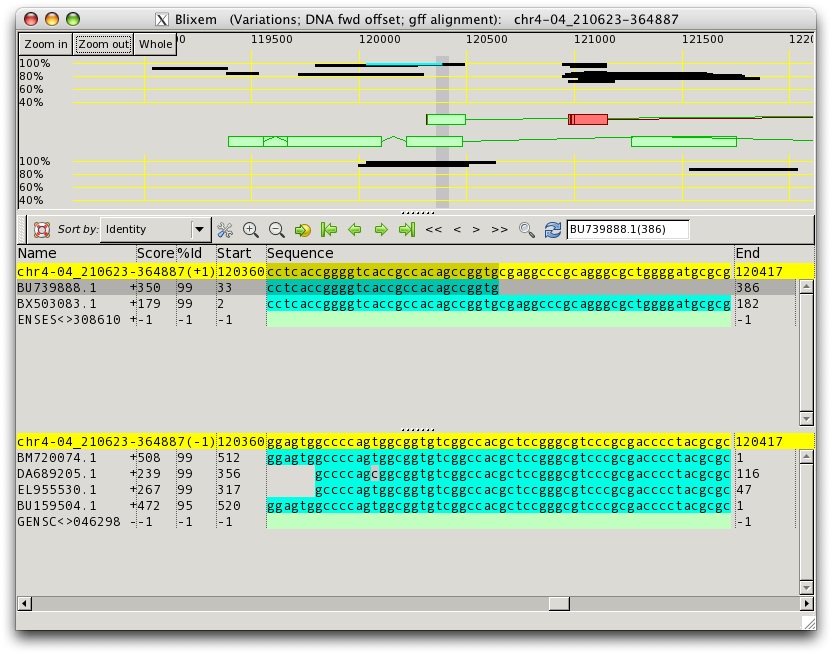
\includegraphics[width=15.231cm,height=11.972cm]{img_window_nucleotide_mode.png}
\caption{Nucleotide mode. There are two panes in the detail-view, one for each strand. 
The active strand is shown at the top. The active strand can be changed by hitting 
the {\textquoteright}Toggle{\textquoteright} button or the
 {\textquoteleft}t{\textquoteright} shortcut key.}
\end{figure}

\begin{figure}
\centering
\color[rgb]{0.30980393,0.5058824,0.7411765}
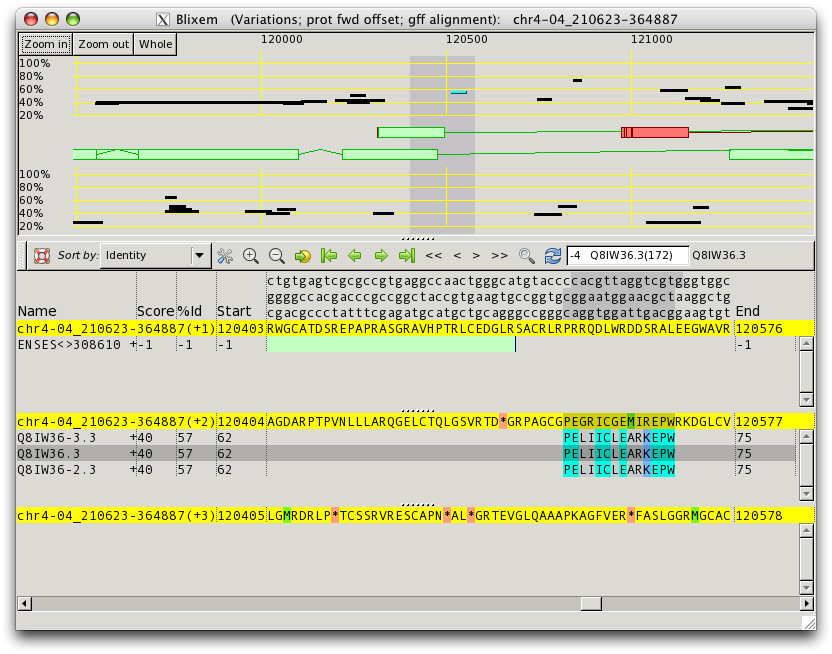
\includegraphics[width=15.231cm,height=11.972cm]{img_window_protein_mode.png}
\caption{Protein mode. There are three
panes in the detail-view; one for each reading frame of the active
strand. The other strand can be activated by hitting the
{\textquoteleft}Toggle{\textquoteright} button or the
{\textquoteleft}t{\textquoteright} shortcut key.}
\end{figure}

\bigskip

{\color[rgb]{0.30980393,0.5058824,0.7411765}\subsection[Active Strand]{Active Strand}}
\hypertarget{RefHeading1621056909880}{}{
The {\textquotedblleft}active{\textquotedblright} reference sequence
strand in Blixem controls the orientation of the display -- coordinates
are shown increasing from left-to-right for the forward strand and
decreasing for the reverse strand. The active strand is always shown
at the top -- i.e. the top grid and top transcript view in the big
picture and the top pane in the detail view.}

\bigskip

In protein mode, only the active strand is shown in the detail view. One must toggle the strand to view the other strand.

\bigskip

{Toggle which strand is active by:}

\liststyleWWviiiNumxxxvi
\begin{itemize}
\item {
pressing the {\textquoteleft}Toggle{\textquoteright} button 

\includegraphics[width=0.496cm,height=0.533cm]{img_button_toggle_strand.png} 
on the toolbar; or}
\item {
pressing the {\textquoteleft}t{\textquoteright} key.}
\end{itemize}

\bigskip

{By default, Blixem assumes that the reference sequence passed to it is
the forward strand, unless otherwise specified by the
{\textquoteleft}-{}-reverse-strand{\textquoteright} command line
argument.}

{\color[rgb]{0.30980393,0.5058824,0.7411765}\subsection[Big Picture]{Big Picture}}
\hypertarget{RefHeading1641056909880}{}{
The {\textquoteleft}Big Picture{\textquoteright} section shows an
overview of the reference sequence. The reference sequence
coordinates are shown along the top. You can zoom in to view a
shorter range by using the {\textquotesingle}Zoom in{\textquotesingle}
button at the top left of the screen. Use {\textquotesingle}Zoom
out{\textquotesingle} or {\textquotesingle}Whole{\textquotesingle} to
zoom out -- {\textquotesingle}Whole{\textquotesingle} zooms out to view
the full length of the reference sequence.}

\bigskip

{The big picture consists of two grids showing the alignments for each
strand, and two sections between these grids showing the transcripts
for each strand. The grids have a scale on the left-hand side showing
the percent-ID, and alignments are plotted against this scale. The
scale and extents of the grids can both be edited - see the Grid
properties section in the Settings dialog.}


\bigskip

{
The active strand alignments and transcripts are shown at the top and
the other strand at the bottom. The direction of the coordinates is
determined by the active strand. The active strand can be toggled
using the {\textquotesingle}t{\textquotesingle} shortcut key or the
{\textquotesingle}Toggle strand{\textquotesingle} button on the
toolbar.}

\bigskip

\begin{figure}
\centering
\color[rgb]{0.30980393,0.5058824,0.7411765}
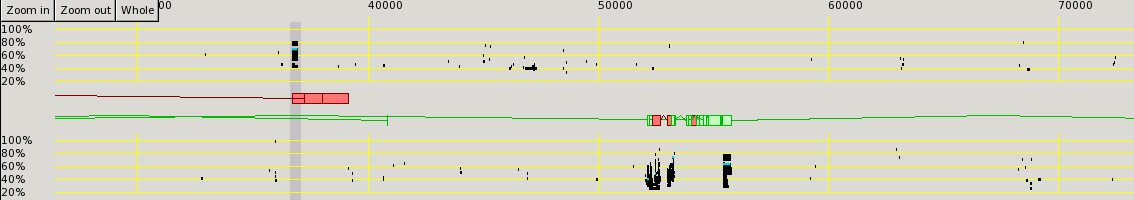
\includegraphics[width=15.24cm,height=2.686cm]{img_view_big_picture.png}
\caption{The Big Picture section}
\end{figure}

{Red shaded areas in the big picture indicate assembly gaps (gaps in the
reference sequence). Assembly gaps are represented by dashes in the
FASTA input file.}

\bigskip

{\color[rgb]{0.30980393,0.5058824,0.7411765}\subsubsection[Bumping the transcript view]{Bumping the transcript view}}
{By default, exons and introns for the same strand are drawn overlapping
each other. They can be expanded (or
{\textquotesingle}bumped{\textquotesingle}) by pressing the
{\textquotesingle}b{\textquotesingle} shortcut key or by enabling the
relevant option in the View dialog (see Hiding sections of the
window).}

\bigskip

\begin{figure}
\centering
\color[rgb]{0.30980393,0.5058824,0.7411765}
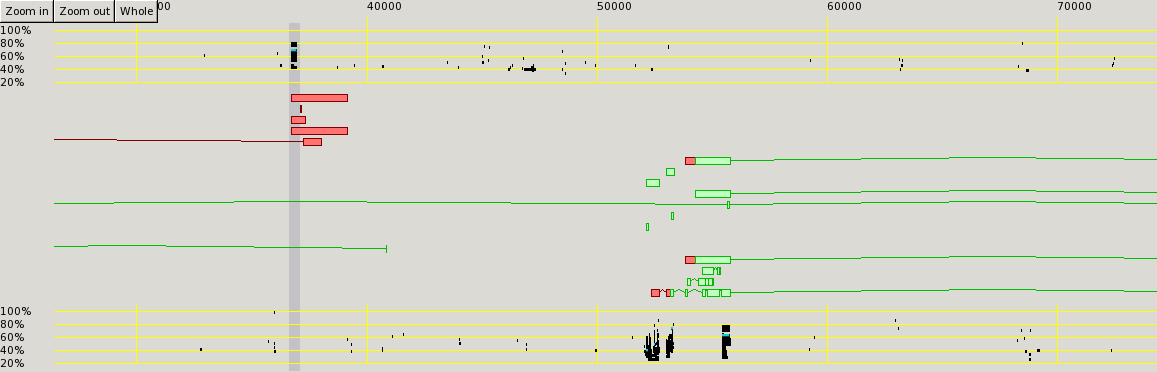
\includegraphics[width=15.24cm,height=4.898cm]{img_view_transcripts.png}
\caption{Expanded transcript view}
\end{figure}

{\color[rgb]{0.30980393,0.5058824,0.7411765}\subsection[Detail View]{Detail View}}
{The {\textquoteleft}Detail View{\textquoteright} shows the actual
sequence data for the match sequences. Match sequences are lined up
underneath the relevant section of reference sequence, and individual
bases are highlighted in different colours to indicate how well they
match.}

\bigskip

{\color[rgb]{0.30980393,0.5058824,0.7411765}\subsubsection[Match colours]{Match colours}}

\begin{figure}
\centering
\color[rgb]{0.30980393,0.5058824,0.7411765}
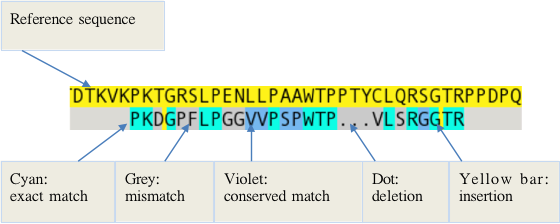
\includegraphics[width=14.353cm,height=5.74cm]{img_view_alignment_colour_key.png}
\caption{ Alignment colour key}
\end{figure}

{\color[rgb]{0.30980393,0.5058824,0.7411765}\subsubsection[Alignment lists]{Alignment lists}}
\hypertarget{RefHeading1701056909880}{}{
There are separate lists of alignments for each strand and reading frame
of the reference sequence. Each list has a yellow header bar
containing the reference sequence. At the left, the yellow bar shows
the reference sequence name and which strand/frame it is, e.g. (+1)
means forward strand, reading frame 1; (-2) means reverse strand,
reading frame 2.}

\begin{figure}
\centering
\color[rgb]{0.30980393,0.5058824,0.7411765}
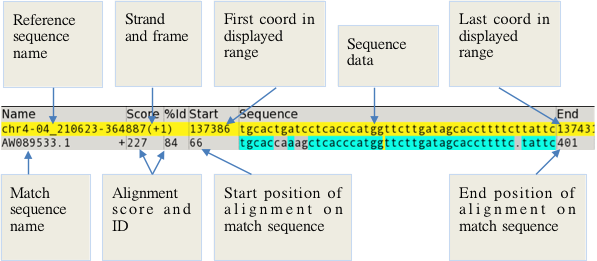
\includegraphics[width=15.288cm,height=6.682cm]{img_view_alignment_details.png}
\caption{Alignment list details}
\end{figure}

\bigskip

{\color[rgb]{0.30980393,0.5058824,0.7411765}\subsubsection[Nucleotide mode]{Nucleotide mode}}
\hypertarget{RefHeading1721056909880}{}{
There are two sections to the detail view in nucleotide mode: one for
each strand. The active strand is shown at the top and defines the
coordinate direction (increasing if the forward strand is active,
decreasing if the reverse is active).}

\begin{figure}
\centering
\color[rgb]{0.30980393,0.5058824,0.7411765}
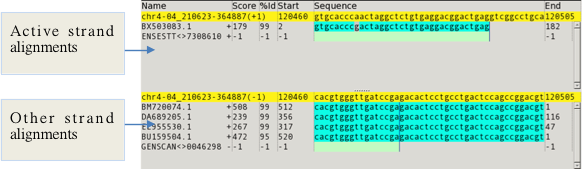
\includegraphics[width=14.933cm,height=4.353cm]{img_view_alignment_details_nucleotide.png}
\caption{Alignment lists: nucleotide mode}
\end{figure}

\bigskip

{\color[rgb]{0.30980393,0.5058824,0.7411765}\subsubsection[Protein mode]{Protein mode}}
\hypertarget{RefHeading1741056909880}{}{
There are three sections in the detail view in protein mode: one for
each of the three reading frames for the active strand. Only the
active strand is shown. To view the other strand, toggle the display
using the {\textquoteleft}Toggle strand{\textquoteright} button or the
{\textquoteleft}t{\textquoteright} shortcut key.}

\bigskip

{In protein mode, the yellow header bars show the translated reference
sequence for that reading frame. STOP and MET codons in the reference
sequence are highlighted in red and green. There is also an
additional header section at the top showing the nucleotide sequence.}

\begin{figure}
\centering
\color[rgb]{0.30980393,0.5058824,0.7411765}
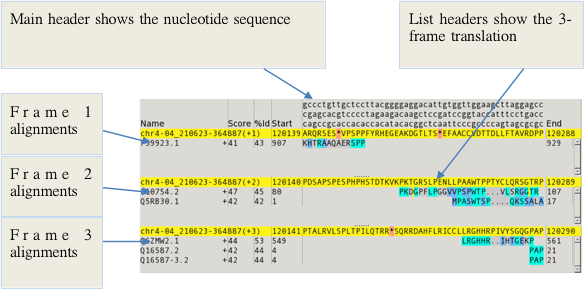
\includegraphics[width=14.974cm,height=7.396cm]{img_view_alignment_details_protein.png}
\caption{Alignment lists: protein mode}
\end{figure}

\bigskip

{In the nucleotide-sequence header, codons are read from top-to-bottom
and then left-to-right, starting at row 1 for frame 1, row 2 for frame
2 etc. Middle-clicking on a coordinate will highlight the three
nucleotides for the selected codon and the currently-active reading
frame (by default, frame 1). Left-clicking in an alignment list sets
the active reading frame.}

\begin{figure}
\centering
\color[rgb]{0.30980393,0.5058824,0.7411765}
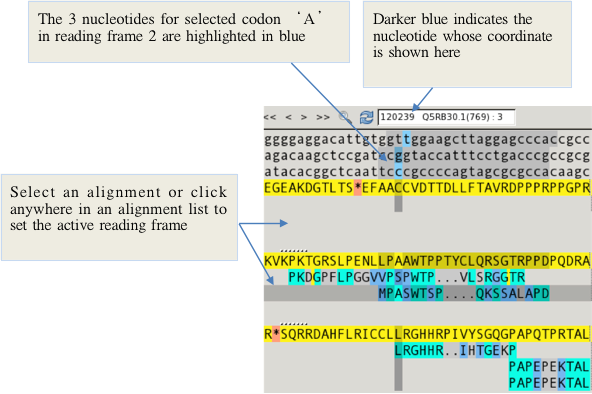
\includegraphics[width=15.177cm,height=10.1cm]{img_view_reading_frame.png}
\caption{Selected reading frame and codon}
\end{figure}

\bigskip

{\color[rgb]{0.30980393,0.5058824,0.7411765}\subsubsection[Exons]{Exons}}
{Exons are displayed as solid-colour blocks in the detail-view, coloured
green for CDS, red for UTR. Vertical blue lines are drawn at the
start and end of the blocks so that it is easy to see whether
alignments line up with the exon boundaries.}

\bigskip

{In protein mode, an exon may not start or end exactly at a codon
boundary. A {\textquotedblleft}partial{\textquotedblright} or
{\textquotedblleft}split{\textquotedblright} codon like this is
indicated in the detail-view by cross-hatch highlighting, and by
drawing a dotted blue line rather than a solid line. (Note that
dotted lines may be obscured by solid lines at the same position.)}

\bigskip

{The true boundary for split codons would really be either a third or
two-thirds of the way through the character width, but Blixem does not
draw boundaries through the middle of characters to avoid too cluttered
a display.}

\begin{figure}
\centering
\color[rgb]{0.30980393,0.5058824,0.7411765}
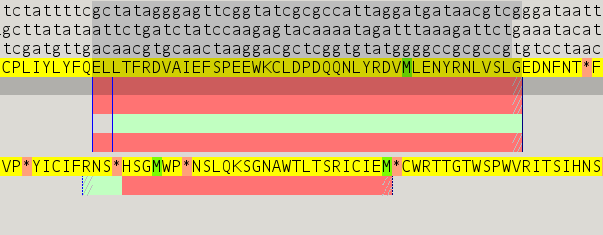
\includegraphics[width=12.321cm,height=4.801cm]{img_view_alignment_list_exons.png}
\caption{Exons in the detail-view.
Split codons are indicated with cross-hatching, e.g. the last codon in
the selected exon is a split codon because it does not include all
three bases for that codon, as you can see from the highlighting in the
DNA header.}
\end{figure}

\bigskip

{\color[rgb]{0.30980393,0.5058824,0.7411765}\subsection[Coverage view]{Coverage view}}
\hypertarget{RefHeading2953469222304}{}{
The coverage view shows a plot of how many alignments there are at each
coordinate along the reference sequence. It can give an indication of
where the regions of interest are.}

\begin{figure}
\centering
\color[rgb]{0.30980393,0.5058824,0.7411765}
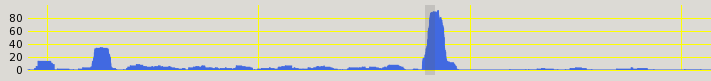
\includegraphics[width=15.24cm,height=1.736cm]{img_view_coverage.png}
\caption{Coverage view}
\end{figure}

\bigskip

{The coverage view can be shown/hidden by ticking/unticking the
{\textquotesingle}Show coverage view{\textquotesingle} check box on the
View dialog (which can be accessed from the right-click menu or by
hitting the {\textquotesingle}v{\textquotesingle} shortcut key).}

\bigskip

{The scale of the coverage view is the same as that of the big-picture
and it can be navigated in the same manner, i.e. }

\liststyleLiv
\begin{itemize}
\item {
use the horizontal scroll-bar or middle-click to scroll; and }
\item {
use the zoom buttons at the top or the Ctrl-=/Ctrl-{}- keys to zoom.}
\end{itemize}

{\color[rgb]{0.30980393,0.5058824,0.7411765}\subsection[The toolbar]{The toolbar}}
{The detail-view toolbar contains the following functions. Note that the
Help and Settings buttons are included in the detail-view toolbar even
though they apply to Blixem as a whole.}

\begin{figure}
\centering
\color[rgb]{0.30980393,0.5058824,0.7411765}

\includegraphics[width=15.24cm,height=0.416cm]{img_toolbar.png}
\caption{Detail-view toolbar}
\end{figure}

\begin{center}
\tablehead{}
\begin{supertabular}{b{1.5cm}p{4.373cm}p{8.967cm}}
 

\includegraphics[width=0.713cm,height=0.7cm]{img_button_help.png} &
\textbf{Help}:  &
Show help about how to use Blixem\\
 

\includegraphics[width=0.73cm,height=0.663cm]{img_button_about.png} &
\textbf{About:} &
Show program information\\
 

\includegraphics[width=0.702cm,height=0.702cm]{img_button_settings.png} &
\textbf{Settings}:  &
Show the Settings dialog\\
 
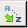
\includegraphics[width=0.661cm,height=0.653cm]{img_button_sort.png} &
\textbf{Sort}:  &
Show the Sort dialog\\
 

\includegraphics[width=0.693cm,height=0.693cm]{img_button_zoom_in.png} &
\textbf{Zoom in}:  &
Increase the font size in the detail-view\\
 

\includegraphics[width=0.693cm,height=0.693cm]{img_button_zoom_out.png} &
\textbf{Zoom out}:  &
Decrease the font size in the detail-view\\
 

\includegraphics[width=0.693cm,height=0.693cm]{img_button_go_to.png} &
\textbf{Go to}: &
Go to a particular coordinate\\
 

\includegraphics[width=0.693cm,height=0.693cm]{img_button_first_match.png} &
\textbf{First match}: &
Go to the first coordinate of the first
alignment\footnotemark[1]\\
 

\includegraphics[width=0.693cm,height=0.693cm]{img_button_prev_match.png} &
\textbf{Previous match}: &
Go to the start of the current alignment or the
end of the previous alignment\footnotemark[1]\\
 

\includegraphics[width=0.693cm,height=0.693cm]{img_button_next_match.png} &
\textbf{Next match}: &
Go to the end of the current alignment or the
start of the next alignment\footnotemark[1]\\
 

\includegraphics[width=0.693cm,height=0.693cm]{img_button_last_match.png} &
\textbf{Last match}: &
Go to the end of the last
alignment\footnotemark[1]\\
 

\includegraphics[width=0.693cm,height=0.693cm]{img_button_back_page.png} &
\textbf{Back one page}: &
Scroll the detail-view range to the left by one
page\\
 

\includegraphics[width=0.536cm,height=0.7cm]{img_button_back_base.png} &
\textbf{Back one index}: &
Scroll the detail-view range to the left by one
base\\
 

\includegraphics[width=0.601cm,height=0.769cm]{img_button_forward_base.png} &
\textbf{Forward one index}: &
Scroll the detail-view range to the right by
one base\\
 

\includegraphics[width=0.693cm,height=0.693cm]{img_button_forward_page.png} &
\textbf{Forward one}\textbf{\textit{
}}\textbf{page}: &
Scroll the detail-view range to the right by
one page\\
 

\includegraphics[width=0.693cm,height=0.693cm]{img_button_find.png} &
\textbf{Find}: &
Scrolls to the start of the first alignment
from that sequence if any are found.\\
 

\includegraphics[width=0.693cm,height=0.751cm]{img_button_toggle_strand.png} &
\textbf{Toggle strand}: &
Toggle which strand is the active strand\\
\end{supertabular}
\end{center}

\footnotetext[1]{Acts only on selected sequences, if there is currently a
selection; if no sequences are currently selected, then this operation
acts on all sequences.}

\bigskip

{\bfseries Feedback box }

{The feedback box contains information about the currently selected
sequence and/or coordinate, if either is selected. Click on a row in
the detail-view to select a sequence. Middle-click on a base in the
detail-view to select that coordinate. Text in the feedback box can
be selected and copied.}

\begin{figure}
\centering
\color[rgb]{0.30980393,0.5058824,0.7411765}
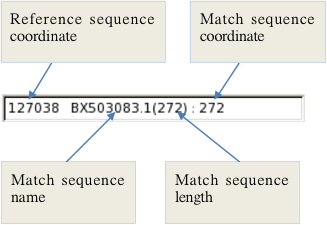
\includegraphics[width=8.359cm,height=5.75cm]{img_view_feedback_box.png}
\caption{Feedback box}
\end{figure}

\bigskip

{\bfseries
Moused-over item feedback area}

The area to the right of the toolbar contains information about the currently moused-over item (e.g. a match sequence in the alignment list or a variation in the variations track). For a match sequence, this information includes the sequence name and optional data such as organism and tissue type that can be parsed from EMBL files. To load optional data, see the Settings dialog. Note that the optional data may be incomplete due to the inconsistent information available from the EMBL files.

\begin{figure}
\centering
\color[rgb]{0.30980393,0.5058824,0.7411765}

\includegraphics[width=7.355cm,height=0.771cm]{img_view_feedback_area.png}
\caption{Moused-over item feedback area}
\end{figure}

\bigskip

{\color[rgb]{0.30980393,0.5058824,0.7411765}\subsection[The main menu]{The main menu}}
\hypertarget{RefHeading1781056909880}{}{
Right-click anywhere in the Blixem window to pop up the main menu.}

\begin{figure}
\centering
\color[rgb]{0.30980393,0.5058824,0.7411765}
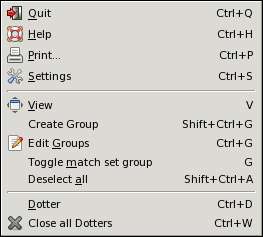
\includegraphics[width=6.951cm,height=6.428cm]{img_menu_right_click.png}
\caption{Main menu}
\end{figure}

{The options are:}

\begin{center}
\tablehead{}
\begin{supertabular}{p{2.9559999cm}p{2.187cm}p{8.343cm}}
\bfseries Quit &
\itshape Ctrl-Q &
 Close Blixem and any spawned processes\\
\bfseries Help &
\itshape Ctrl-H &
 Display the user help\\
 \textbf{Print}  &
\itshape Ctrl-P &
 Printing options\\
\bfseries Settings &
\itshape Ctrl-S &
 Edit settings\\
 \textbf{View}  &
\itshape v &
 Show/hide parts of the display\\
\bfseries Create Group &
\itshape Shift-Ctrl-G &
 Create a group of sequences\\
 \textbf{Edit Groups}  &
\itshape Ctrl-G &
 Edit properties for groups\\
\bfseries Toggle match set group &
\itshape G &
 Toggle the special {\textquotedblleft}match
set{\textquotedblright} group on and off. This is a quick way of
creating a group from the current selection buffer, which should
contain match sequence names.\\
\bfseries Deselect all &
\itshape Shift-Ctrl-A &
 Deselect all sequences\\
 \textbf{Dotter}  &
\itshape Ctrl-D &
 Run Dotter on the currently selected sequence\\
\bfseries Close all Dotters &
~
 &
 Close all Dotters that have been opened from
this Blixem\\
\end{supertabular}
\end{center}

{\color[rgb]{0.30980393,0.5058824,0.7411765}\subsection[Hiding sections of the window]{Hiding sections of the window}}
\hypertarget{RefHeading1801056909880}{}\label{bkm:RefHeading1801056909880}{
Use to {\textquoteleft}View{\textquoteright} dialog to show/hide
sections of the window.}

\liststyleWWviiiNumxxxi
\begin{enumerate}
\item {
Right-click and select the View option, or hit the
{\textquoteright}v{\textquoteright} shortcut key.}
\item {
Toggle check marks on or off to show/hide sections.}
\end{enumerate}

\begin{figure}
\centering
\color[rgb]{0.30980393,0.5058824,0.7411765}
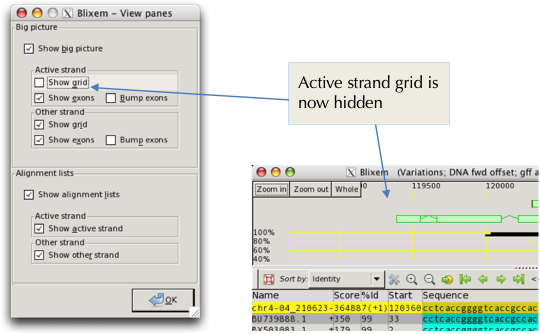
\includegraphics[width=13.818cm,height=8.546cm]{img_dialog_view.png}
\caption{The View dialog}
\end{figure}

\bigskip

{Alternatively, use the following keyboard shortcuts to toggle visibility
of a component:}

\begin{center}
\tablehead{}
\begin{supertabular}{p{2.289cm}p{11.909cm}}
\bfseries 1 &
 Hide top pane in detail view\\
\bfseries 2 &
 Hide second pane in detail view\\

{\textbf{3}}{ } &
 Hide third pane in detail view (protein mode
only)\\

{\textbf{Ctrl-1}}{ }
&
 Hide top grid in big picture (active strand)\\

{\textbf{Ctrl-2}}{ }
&
 Hide bottom grid in big picture (other
strand)\\

{\textbf{Shift-Ctrl-1}}{
} &
 Hide top exon view (active strand)\\

{\textbf{Shift-Ctrl-2}}{
} &
 Hide bottom exon view (other strand)\\
\end{supertabular}
\end{center}

{\color[rgb]{0.0,0.27058825,0.5254902}\section[Operation]{Operation}}
{\color[rgb]{0.30980393,0.5058824,0.7411765}\hypertarget{RefHeading1821056909880}{}\subsection[Navigation]{Navigation}}
{\color[rgb]{0.30980393,0.5058824,0.7411765}\hypertarget{RefHeading1841056909880}{}\subsubsection[Scrolling]{Scrolling}}
\hypertarget{RefHeading1861056909880}{}\begin{flushleft}
\tablehead{}
\begin{supertabular}{p{4.15cm}p{10.436cm}}
{\bfseries Middle-click/double-click and then
drag in big picture}

~
 &
 Jump to a particular region. Dragging moves the highlight box.\\
{\bfseries Click on the highlight box and drag}

~
 &
 Move the highlight box.\\
{\bfseries Middle-click/drag in detail view}

~
 &
 Select a base. Releasing the mouse button scrolls the display to centre on the selected base (hold down Ctrl to avoid scrolling.)\\
\bfseries Click a feature in the big picture &
{ Selects that feature and scrolls the
detail-view vertically so that it is visible (if it is in the current
detail view range).}

~
\\
{\bfseries Horizontal scrollbar}

~
 &
 Scroll the detail-view range.\\
{\bfseries Vertical scrollbars}

~
 &
 Scroll up/down in the detail view or the big
picture.\\
{\bfseries Horizontal mouse-wheel}

~
 &
{ Scroll the detail-view range (if your mouse
has a horizontal scroll-wheel).}

~
\\
{\bfseries Vertical mouse-wheel}

~
 &
{ Scroll up/down the currently moused-over
alignment list in the detail view, or the big picture.}

~
\\
{\bfseries Ctrl-left}

{\bfseries Ctrl-right}

~
 &
{ Scroll to the start/end of the previous/next
match (limited to currently-selected sequences, if any are selected;
includes all sequences otherwise).}

~
\\
{\bfseries Home}

{\bfseries End}

~
 &
 Scroll to the start/end of the display.\\
{\bfseries Ctrl-Home}

{\bfseries Ctrl-End}

~
 &
{ Scroll to the start/end of the
currently-selected alignments (or to the first/last alignment if none
are selected).}

~
\\
{\bfseries {\textquoteleft},{\textquoteright}
(comma)}

{\bfseries {\textquoteleft}.{\textquoteright}
(full-stop)}

~
 &
 Scroll the detail-view range one nucleotide to
the left/right.\\
{\bfseries Ctrl-,}

{\bfseries Ctrl-.}

~
 &
 Scroll the detail-view range one page to the
left/right.\\
{\bfseries Go-to button or}

\bfseries {\textquoteleft}p{\textquoteright} key
&
 Scroll to a specific coordinate position.\\
\end{supertabular}
\end{flushleft}

{\color[rgb]{0.30980393,0.5058824,0.7411765}\subsubsection[Zooming]{Zooming}}
\hypertarget{RefHeading1881056909880}{}\begin{flushleft}
\tablehead{}
\begin{supertabular}{p{4.801cm}p{9.729cm}}
{ \textbf{= \ {}- \ keys and }

\includegraphics[width=0.653cm,height=0.653cm]{img_button_zoom_in.png} 

\includegraphics[width=0.653cm,height=0.653cm]{img_button_zoom_out.png}
\textbf{ }}

~
 &
 Zoom in/out of the detail-view\\
{\bfseries Ctrl-= or Ctrl-{}- keys and}

 
\includegraphics[width=1.404cm,height=0.635cm]{img_button_zoom_in_bp.png} 
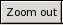
\includegraphics[width=1.603cm,height=0.647cm]{img_button_zoom_out_bp.png} 

~
 &
 Zoom in/out of the big-picture\\
 \textbf{Shift-Ctrl-{}- and }
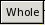
\includegraphics[width=1.289cm,height=0.723cm]{img_button_zoom_whole_bp.png} 
&
 Zoom the big picture out to view the full
length of the reference sequence.\\
\end{supertabular}
\end{flushleft}

{\color[rgb]{0.30980393,0.5058824,0.7411765}\subsection[Selections]{Selections}}
\hypertarget{RefHeading1901056909880}{}
{\color[rgb]{0.30980393,0.5058824,0.7411765}\subsubsection[Selecting sequences]{Selecting sequences}}
\hypertarget{RefHeading1921056909880}{}
\liststyleWWviiiNumxxxv
\begin{itemize}
\item {You can select a sequence by clicking on its row in the alignment list. Selected sequences are highlighted in cyan in the big picture.}
\item {You can select a sequence by clicking on it in the big picture.}
\item {The name of the sequence you selected is displayed in the feedback box on the toolbar. If there are multiple alignments for the same sequence, all of them will be selected.}
\item {You can select multiple sequences by holding down the Ctrl or Shift keys while selecting rows.}
\item {You can deselect a single sequence by Ctrl-clicking on its row.}
\item {You can deselect all sequences by right-clicking and selecting {\textquotesingle}Deselect all{\textquotesingle}, or with the Shift-Ctrl-A keyboard shortcut.}
\item {You can move the selection up/down a row using the up/down arrow keys.}
\end{itemize}

{\color[rgb]{0.30980393,0.5058824,0.7411765}\subsubsection[Selecting coordinates]{Selecting coordinates}}
\hypertarget{RefHeading1941056909880}{}

\begin{figure}
\centering
\color[rgb]{0.30980393,0.5058824,0.7411765}
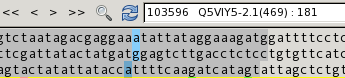
\includegraphics[width=9.904cm,height=2.244cm]{img_view_selected_codon.png}
\caption{ The 3 nucleotides for the
currently-selected amino acid in reading-frame 3. Selected nucleotide
103596 is shaded in darker blue.}
\end{figure}

\liststyleWWviiiNumxiii
\begin{itemize}
\item {
You can select a nucleotide/peptide by middle-clicking on it in the
detail view. This selects the entire column at that index, and the
coordinate number on the reference sequence is shown in the feedback
box. (The coordinate on the match sequence is also shown if a match
sequence is selected.)}
\item {
By default the display will centre on the selected base when you middle
click. To select a base without scrolling, hold down Ctrl when you
middle click.}
\item {
For protein matches, when a peptide is selected, the three nucleotides
for that peptide (for the active reading frame) are highlighted in the
header in blue. (The active reading frame is whichever alignment list
currently has the focus - click in a different list to change the
reading frame.) Darker blue highlighting indicates the specific
nucleotide that is currently selected (i.e. whose coordinate is
displayed in the feedback box).}
\item {
You can move the selection to the previous/next index using the left and
right arrow keys.}
\item {
In protein mode, you can move the selected nucleotide by a single base
(rather than an entire codon) holding Shift while using the left and
right arrow keys.}
\item {
You can move the selection to the start/end of the previous/next match
by holding Ctrl while using the left and right arrow keys (limited to
just the selected sequences if any are selected; includes all sequences
otherwise).}
\end{itemize}

{\color[rgb]{0.30980393,0.5058824,0.7411765}\subsubsection[Finding sequences]{Finding sequences}}
\hypertarget{RefHeading1961056909880}{}{
The Find dialog allows the user to search for sequences by name. Press
the Find 

\includegraphics[width=0.487cm,height=0.487cm]{img_button_find.png} 
button on the toolbar or hit the
{\textquoteleft}Ctrl-F{\textquoteright} shortcut key to open the Find
dialog.}

\begin{figure}
\centering
\color[rgb]{0.30980393,0.5058824,0.7411765}
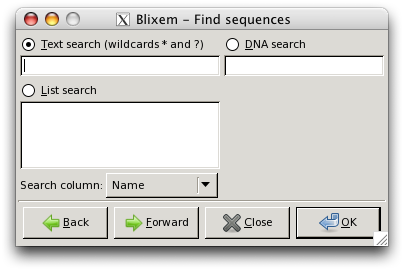
\includegraphics[width=11.037cm,height=7.103cm]{img_dialog_find.png}
\caption{Find dialog}
\end{figure}

\bigskip

{There are three search modes:}

\liststyleWWviiiNumxxvii
\begin{itemize}
\item {
Text search: Search for match sequences by name (or another column from
the {\textquotesingle}Search column{\textquotesingle} drop-down box).
The wild-card {\textquoteleft}*{\textquoteright} means any number (or
zero) of any character and {\textquoteleft}?{\textquoteright} means 1
character (which can be any character). Any sequences whose relevant
column data matches the search string will be selected and the display
will scroll to the start of the selection. }
\item {
List search: the same as text-search, but you can enter multiple search
strings by placing them on separate lines in the text box.}
\item {
DNA search: This searches for a given sub-sequence of nucleotides in the
reference sequence. If the sub-sequence is found, the display will
scroll to the start of the sub-sequence and the first base in the
sub-sequence will be selected.}
\end{itemize}

{Enter your search text in the appropriate box and click the OK button to
perform the search. By default, Blixem will start searching from the
beginning of the reference sequence range. To start the search from
the current position instead, click the Forward or Back button instead
of OK. This will start searching from the currently-selected base, if
there is one selected; if not, it will start from the beginning of the
current detail-view display range when searching forwards or from the
end of the display range if searching backwards.}


\bigskip

{\bfseries
Repeat a Find}

After clicking OK on the Find dialog, press F3 to repeat the search in a
forwards direction or Shift-F3 to repeat in a backwards direction.
Alternatively, if you had selected the Forward or Back button in the
Find dialog then click the Forward or Back buttons again to jump to the
next result in that direction.

{\color[rgb]{0.30980393,0.5058824,0.7411765}\subsubsection[Copy and paste]{Copy and paste}}
\hypertarget{RefHeading1981056909880}{}\liststyleWWviiiNumxxvi
\begin{itemize}
\item {
When sequence(s) are selected, their names are copied to the
\textit{selection buffer }and can be pasted to another program by
middle-clicking in that program.}
\item {
Sequence names can be pasted from the selection buffer into Blixem by
hitting the {\textquotesingle}f{\textquotesingle} keyboard shortcut. If
the selection buffer contains valid sequence names, those sequences
will be selected and the display will jump to the start of the
selection.}
\item {
Sequence names can also be pasted from the selection buffer into text
boxes in dialog boxes such as the Groups dialog or Find dialog.}
\item {
To copy sequence name(s) to the \textit{default clipboard}, select the
sequence(s) and hit Ctrl-C. Sequence names can then be pasted into
other applications using Ctrl-V.}
\item {
The default clipboard can be pasted into Blixem using Ctrl-V. If the
clipboard contains valid sequence names, those sequences will be
selected and the display will jump to the start of the selection.}
\item {
Note that text from the feedback box and some text labels (e.g. the
reference sequence start/end coords) can be copied to the selection
buffer by selecting the required text with the mouse (or copied to the
default clipboard by selecting it and then hitting
{\textquoteleft}Ctrl-C{\textquoteright}).}
\item {
Text can be pasted from the default clipboard into text entry boxes on
dialogs such as the Groups or Find dialog by using Ctrl-V.}
\end{itemize}

{\color[rgb]{0.30980393,0.5058824,0.7411765}\subsection[Sorting alignments]{Sorting alignments}}
\hypertarget{RefHeading2001056909880}{}\liststyleWWviiiNumxxvi

\begin{figure}
\centering
\color[rgb]{0.30980393,0.5058824,0.7411765}
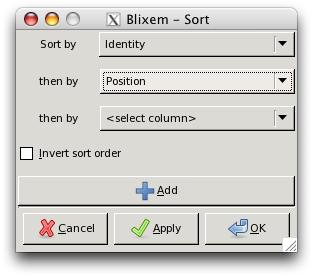
\includegraphics[width=8.881cm,height=7.602cm]{img_dialog_sort.png}
\caption{Sort dialog}
\end{figure}

\liststyleWWviiiNumxxvi
\begin{itemize}
\item {Click the sort button on the toolbar to open the Sort dialog.}
\item {Select the column you wish to sort by from the top drop-down box on the dialog.}
\item {You may optionally sort by further columns. You can sort by as many columns as you wish by adding further drop-down boxes using the Add button.}
\item {The default sort order may be ascending or descending depending on what makes most sense for the selected column: e.g. sorting by position is \textit{ascending} by default, but sorting by score or ID is \textit{descending}.}
\item {To get the inverse of the default sort order, select the {\textquoteleft}Invert sort order{\textquoteright} option on the Sort dialog.}
\item {Alignments can also be sorted by group. Alignments that are part of a group will then be listed first (before any that are not in a group), and ordered according to the group{\textquoteright}s order number. See the Groups section for more details.}
\end{itemize}

\begin{figure}
\centering
\color[rgb]{0.30980393,0.5058824,0.7411765}
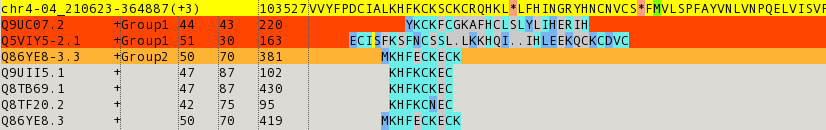
\includegraphics[width=13.721cm,height=2.164cm]{img_view_sort_by_group.png}
\caption{Alignment list sorted by group}
\end{figure}

\bigskip

{\color[rgb]{0.30980393,0.5058824,0.7411765}\subsection[Fetching sequences]{Fetching sequences}}
\hypertarget{RefHeading2021056909880}{}

\liststyleWWviiiNumxvi
\begin{itemize}
\item {Double-click a row to fetch a match sequence{\textquoteright}s EMBL
file.}
\end{itemize}

{\color[rgb]{0.30980393,0.5058824,0.7411765}\subsection[Grouping sequences]{Grouping sequences}}
\hypertarget{RefHeading2041056909880}{}{
Alignments can be grouped together so that they can be
sorted/highlighted/hidden etc.}

{\color[rgb]{0.30980393,0.5058824,0.7411765}\subsubsection[Creating a group from a selection]{Creating a group from a selection}}
\hypertarget{RefHeading2061056909880}{}\liststyleWWviiiNumxvi
\begin{itemize}
\item {Select the sequences you wish to include in the group by left-clicking their rows in the detail view. Multiple rows can be selected by holding the Ctrl or Shift keys while clicking.}
\item {Right-click and select {\textquotesingle}Create Group{\textquotesingle}, or use the Shift-Ctrl-G shortcut key. (Note that Ctrl-G will also shortcut to here if no groups currently exist.)}
\item {Ensure that the {\textquotesingle}From selection{\textquotesingle} radio button is selected, and click {\textquotesingle}OK{\textquotesingle} or {\textquoteleft}Apply{\textquoteright}. If you click {\textquoteleft}Apply{\textquoteright}, you will be shown the group you just created so that you can edit it. If you click {\textquoteleft}OK{\textquoteright} the group will be created with the
default properties.}
\end{itemize}

\begin{figure}
\centering
\color[rgb]{0.30980393,0.5058824,0.7411765}
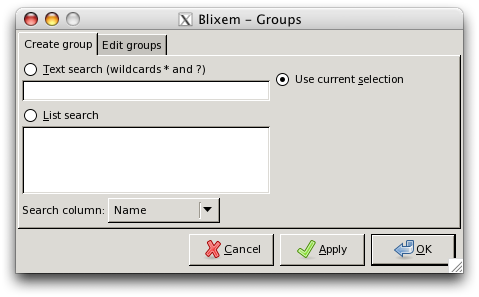
\includegraphics[width=11.95cm,height=7.084cm]{img_dialog_groups.png}
\caption{Groups dialog - create group}
\end{figure}

{\color[rgb]{0.30980393,0.5058824,0.7411765}\subsubsection[Creating a group from a search]{Creating a group from a search}}
\hypertarget{RefHeading33212258250716}{}\liststyleWWviiiNumxvi
\begin{itemize}
\item {
Right-click and select {\textquotesingle}Create Group{\textquotesingle},
or use the Shift-Ctrl-G shortcut key. (Or Ctrl-G if no groups currently
exist.)}
\item {
Select the {\textquotesingle}Text search{\textquotesingle} or
{\textquotesingle}List search{\textquotesingle} radio button and enter
some text to search for.}
\item {
Select the column that you wish to search in the drop-down box at the
bottom.}
\item {
Click OK or Apply.}
\end{itemize}

\bigskip

{\bfseries
Notes}

\liststyleWWviiiNumxvi
\begin{itemize}
\item {{\textquotesingle}List search{\textquotesingle} allows you to enter multiple search strings; place each string on a separate line.}
\item {You can use the following wild-cards in the search text: an asterisk (*) represents any number of characters; a question mark (?) represents any single character.}
\item {You can paste text into the search boxes from the selection buffer by middle-clicking or from the clipboard using Ctrl-V.}
\item {You may paste sequence names directly from another compatible program (e.g. ZMap): click on the feature in ZMap and then middle-click in the text box on the Groups dialog. (Grouping in Blixem works on the sequence name alone, so the feature coords output by ZMap will be ignored.)}
\end{itemize}

{\color[rgb]{0.30980393,0.5058824,0.7411765}\subsubsection[Creating a temporary
{\textquotesingle}match{}-set{\textquotesingle} group from the current
selection]{Creating a temporary
{\textquotesingle}match-set{\textquotesingle} group from the current
selection}}
\hypertarget{RefHeading2121056909880}{}\liststyleWWviiiNumxvi
\begin{itemize}
\item {You can quickly create a group from a current selection (e.g. selected features in ZMap or just the current selection in Blixem) using the {\textquotesingle}Toggle match set{\textquotesingle} option.}
\item {To create a match-set group, select the required items and then select {\textquotesingle}Toggle match set{\textquotesingle} from the right-click menu in Blixem, or hit the {\textquotesingle}g{\textquotesingle} shortcut key.}
\item {To clear the match-set group, choose the {\textquotesingle}Toggle match set{\textquotesingle} option again, or hit the {\textquotesingle}g{\textquotesingle} shortcut key again.}
\item {While it is enabled (i.e. toggled on), the match-set group can be edited like any other group, via the {\textquotesingle}Edit Groups{\textquotesingle} dialog. Any settings you change (e.g. highlight colour) will be saved even if the match-set group is toggled off and then on again.}
\item {If you delete the match-set group using the {\textquotesingle}Edit Groups{\textquotesingle} dialog, all of its settings will be lost; you will get the default settings again the next time you enable the match-set group. To avoid this, disable it by toggling it off using the {\textquotesingle}Toggle match set{\textquotesingle} menu option (or {\textquotesingle}g{\textquotesingle} shortcut key) rather than by deleting it in the Groups dialog.}
\end{itemize}

{\color[rgb]{0.30980393,0.5058824,0.7411765}\subsubsection[Editing groups]{Editing groups}}
\hypertarget{RefHeading2141056909880}{}{
To edit a group, right-click and select {\textquotesingle}Edit
Groups{\textquotesingle}, or use the Ctrl-G shortcut key.}

\begin{figure}
\centering
\color[rgb]{0.30980393,0.5058824,0.7411765}
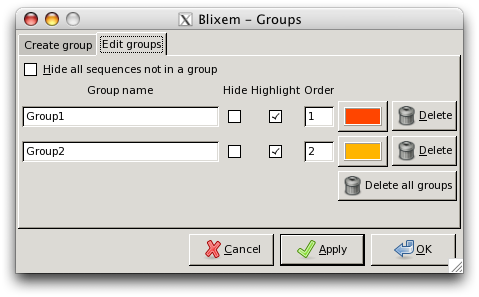
\includegraphics[width=12.746cm,height=7.394cm]{img_dialog_groups_edit.png}
\caption{Groups dialog -- edit groups}
\end{figure}

You can change the following properties for a group. Click on Apply or OK to apply the changes.

\bigskip

\begin{flushleft}
\tablehead{}
\begin{supertabular}{p{3.1069999cm}p{11.479cm}}
\bfseries Name &
 You can specify a more meaningful name to help
you identify the group.\\
\bfseries Hide &
 Tick this box to hide the alignments in the
alignment lists.\\
\bfseries Highlight &
 Tick this box to highlight the alignments.\\
\bfseries Colour &
 The colour the group will be highlighted in, if
{\textquotesingle}Highlight{\textquotesingle} is enabled. The default
colour for all groups is orange, so you may wish to change this if you
want different groups to be highlighted in different colours.\\
\bfseries Order &
 When sorting by Group, alignments in a group
with a lower order number will appear before those with a higher order
number (or vice versa if sort order is inverted). Alignments in a group
will appear before alignments that are not in a group.\\
\end{supertabular}
\end{flushleft}

\bigskip

You can also hide all sequences that are not part of a group by ticking the {\textquotesingle}Hide all sequences not in a group{\textquotesingle} option. This is a quick way of filtering sequences to show only those that you are interested in; any sequences that are not part of a group will be hidden. Note that any sequences in a hidden group will also still be hidden.


\bigskip

To delete a group, click one of the following buttons. This will have an immediate effect (i.e. you don{\textquoteright}t have to click {\textquoteleft}Apply{\textquoteright}).

\liststyleWWviiiNumxxxvii
\begin{itemize}
\item {
To delete a single group, click on the
{\textquotesingle}Delete{\textquotesingle} button next to the group you
wish to delete.}
\item {
To delete all groups, click on the {\textquotesingle}Delete all
groups{\textquotesingle} button.}
\end{itemize}
{\color[rgb]{0.30980393,0.5058824,0.7411765}\subsection[Running dotter]{Running dotter}}
\hypertarget{RefHeading2161056909880}{}\liststyleWWviiiNumxxxvii
\begin{itemize}
\item {
To start Dotter from within Blixem, or to edit the parameters for
running Dotter, right-click and select
{\textquotesingle}Dotter{\textquotesingle} or use the Ctrl-D keyboard
shortcut. The Dotter dialog will pop up.}
\end{itemize}

\begin{figure}
\centering
\color[rgb]{0.30980393,0.5058824,0.7411765}
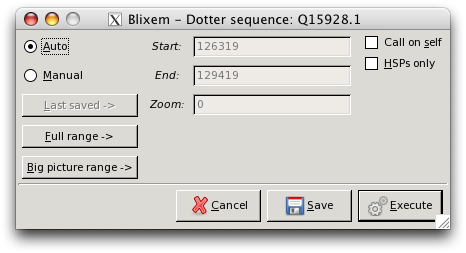
\includegraphics[width=13.215cm,height=7.165cm]{img_dialog_dotter.png}
\caption{Dotter dialog}
\end{figure}

\liststyleWWviiiNumxxxvii
\begin{itemize}
\item {Select the sequence you wish to run Dotter on before or after opening the dialog. The selected sequence name will be shown at the top of the dialog.}
\item {Alternatively, if you just wish to edit the settings, you do not need to select a sequence.}
\item {To run Dotter with the default (automatic) parameters, just hit RETURN, or click the {\textquotesingle}Execute{\textquotesingle} button.}
\item {To enter custom parameters, select the {\textquotesingle}Manual{\textquotesingle} radio button and enter the values in the {\textquotesingle}Start{\textquotesingle} and {\textquotesingle}End{\textquotesingle} boxes.}
\item {To save the parameters without running Dotter, click Save and then Cancel{\textquotesingle}.}
\item {To save the parameters and run Dotter, click {\textquotesingle}Execute{\textquotesingle}.}
\item {To revert to the last-saved manual parameters, click the {\textquotesingle}Last saved{\textquotesingle} button.}
\item {To revert back to automatic parameters, click the {\textquotesingle}Auto{\textquotesingle} radio button. The coordinates in the Start and End box will be recalculated for the currently-selected sequence.}
\end{itemize}
{\color[rgb]{0.30980393,0.5058824,0.7411765}\subsubsection[Reference sequence versus itself]{Reference sequence versus itself}}
\hypertarget{RefHeading2181056909880}{}
To run Dotter on the reference sequence versus itself, select the {\textquoteleft}Call on self{\textquoteright} tick box in the Dotter dialog and then click {\textquoteleft}Execute{\textquoteright}. This can be useful to analyse internal repeats etc. (see the Dotter manual for more information).

\bigskip

{\color[rgb]{0.30980393,0.5058824,0.7411765}\subsubsection[Dotter HSPs only]{Dotter HSPs only}}
\hypertarget{RefHeading2201056909880}{}{
This starts Dotter in HSP (High-Scoring Pair) mode (see the Dotter
manual).}

\bigskip

{\color[rgb]{0.0,0.27058825,0.5254902}\section[Settings]{Settings}}
\hypertarget{RefHeading2221056909880}{}
The settings menu can be accessed by right-clicking and selecting Settings, or by the shortcut Ctrl-S.

{\color[rgb]{0.30980393,0.5058824,0.7411765}\subsection[Features]{Options}}
\hypertarget{RefHeading2241056909880}{}
{\color[rgb]{0.30980393,0.5058824,0.7411765}\subsubsection[Highlight variations]{Highlight variations}}
\hypertarget{RefHeading2261056909880}{}
When this option is enabled, bases in the reference sequence that have know variations (such as SNPs, insertions, deletions etc., loaded from the GFF file) are highlighted in the reference sequence (nucleotide) header.

\bigskip

If the {\textquoteleft}Show variations track{\textquoteright} sub-option is also enabled, then an additional line is shown above the nucleotide header showing the alternative bases for each variation. Note that the Variations track can be quickly enabled or disabled by double-clicking the nucleotide header.

\bigskip

You can double-click a variation to open its URL.

\begin{figure}
\centering
\color[rgb]{0.30980393,0.5058824,0.7411765}
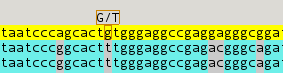
\includegraphics[width=7.181cm,height=1.852cm]{img_view_variations.png}
\caption{Variations track}
\end{figure}

\bigskip

{\color[rgb]{0.30980393,0.5058824,0.7411765}\subsubsection[Show polyA tails]{Show polyA tails}}
\hypertarget{RefHeading2281056909880}{}
When this option is enabled, polyA tails are shown and highlighted in the alignment lists and polyA signals are highlighted in the reference sequence (nucleotide) header. If the sub-option {\textquoteleft}Selected sequences only{\textquoteright} is enabled, polyA tails will only be shown for the currently selected sequences.

\bigskip

Annotated polyA sites and signals form the input features file are also highlighted in the reference sequence. Mouse-over an annotated site/signal to see its details.

\bigskip

{\color[rgb]{0.30980393,0.5058824,0.7411765}\subsubsection[Show Unaligned Sequence ]{Show Unaligned Sequence }}
\hypertarget{RefHeading2321056909880}{}
When this option is enabled, any additional, unaligned portions of the match sequences are displayed at the start and end of the alignments. If the {\textquoteleft}Limit to{\textquoteright} sub-option is also enabled, you can specify the maximum number of additional bases to display. If the {\textquoteleft}Selected sequences only{\textquoteright} sub-option is enabled, only the currently selected sequence(s) will display unaligned portions of sequence.

\bigskip

{\color[rgb]{0.30980393,0.5058824,0.7411765}\subsubsection[Show Colinearity Lines ]{Show Colinearity Lines }}
\hypertarget{RefHeading2321056909880}{}
When this option is enabled, colinearity lines are displayed between alignment blocks of the same sequence. The lines are green to indicate perfectly colinear, orange to indicate imperfectly colinear, and red to indicate not colinear. If the {\textquoteleft}Selected sequences only{\textquoteright} sub-option is enabled, colinearity lines are only displayed for the currently selected sequence(s) in the detail view, otherwise they are shown for all sequences in the detail view. Note that colinearity lines are only displayed for the selected sequence(s) in the big picture regardless of this setting, to save cluttering the screen.
\bigskip

{\color[rgb]{0.30980393,0.5058824,0.7411765}\subsubsection[Show Splice Sites]{Show Splice Sites}}
\hypertarget{RefHeading2341056909880}{}
When this option is enabled, splice sites are highlighted in the reference sequence (nucleotide) header for the currently-selected sequence(s). The two bases from the adjacent introns are highlighted in green if they are canonical or red if they are non-canonical.

\begin{figure}
\centering
\color[rgb]{0.30980393,0.5058824,0.7411765}
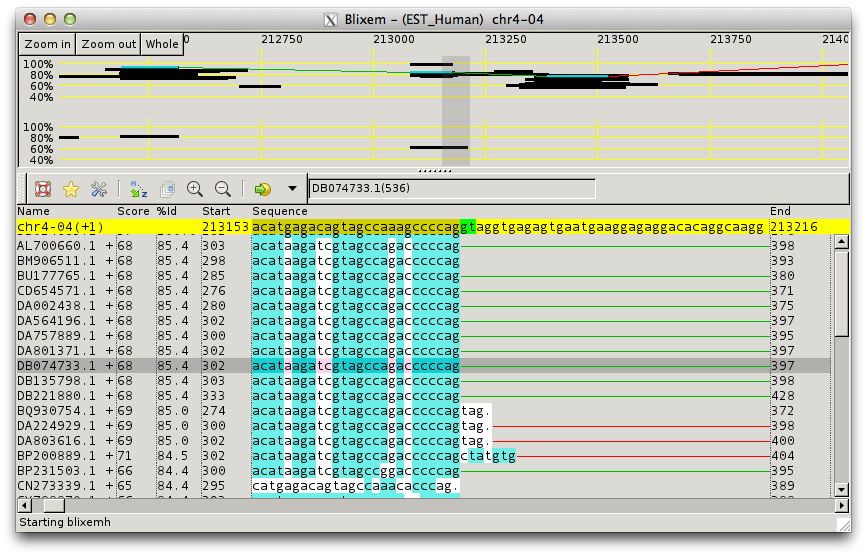
\includegraphics[width=\textwidth]{img_view_colinearity.png}
\caption{Colinearity lines between alignment blocks and highlighted splice-sites in the reference sequence}
\end{figure}

\bigskip

{\color[rgb]{0.30980393,0.5058824,0.7411765}\subsubsection[Highlight Differences]{Highlight Differences}}
\hypertarget{RefHeading2361056909880}{}
When this option is enabled, matching bases are blanked out and mismatches are highlighted, making it easier to see where alignments differ from the reference sequence.

\bigskip

{\color[rgb]{0.30980393,0.5058824,0.7411765}\subsubsection[Squash Matches ]{Squash Matches }}
\hypertarget{RefHeading2381056909880}{}
This groups multiple alignments from the same sequence together into the same row in the detail view, rather than showing them on separate rows.

\bigskip

{\color[rgb]{0.30980393,0.5058824,0.7411765}\subsection[Display]{Display}}
\hypertarget{RefHeading2421056909880}{}
{\color[rgb]{0.30980393,0.5058824,0.7411765}\subsubsection[Use print colours]{Use print colours}}
\hypertarget{RefHeading2641056909880}{}
Select this option to make Blixem use grey-scale colours, suitable for printing.

\bigskip

{\color[rgb]{0.30980393,0.5058824,0.7411765}\subsubsection[Font]{Font}}
\hypertarget{RefHeading2441056909880}{}
Allows you to change the font that is used to display alignments in the detail-view. Note that you must select a monospace font; otherwise matches will not be shown aligned correctly. Blixem will warn you if the font you have selected is not monospace.

\bigskip

{\color[rgb]{0.30980393,0.5058824,0.7411765}\subsubsection[\%ID per cell]{\%ID per cell}}
\hypertarget{RefHeading2561056909880}{}
Use this to change the vertical scale of the big picture grid; a smaller value means the grid will be more spaced out, a larger value means the grid will be more compact.

\bigskip

{\color[rgb]{0.30980393,0.5058824,0.7411765}\subsubsection[Max \%ID]{Max \%ID}}
\hypertarget{RefHeading2581056909880}{}
Defines the maximum cut-off value for the \%ID scale in the big picture grid.

\bigskip

{\color[rgb]{0.30980393,0.5058824,0.7411765}\subsubsection[Min \%ID]{Min \%ID}}
\hypertarget{RefHeading2601056909880}{}
Defines the minimum cut-off value for the \%ID scale in the big picture grid.

\bigskip

{\color[rgb]{0.30980393,0.5058824,0.7411765}\subsubsection[Depth per cell]{Depth per cell}}
\hypertarget{RefHeading334716266717}{}
Use this to change the vertical scale of the grid for the Coverage View (see the View menu to turn on the Coverage View); a smaller value means the grid will be more spaced out, a larger value means the grid will be more compact.

\bigskip

{\color[rgb]{0.30980393,0.5058824,0.7411765}\subsection[Columns]{Columns}}
\hypertarget{RefHeading2481056909880}{}
{\color[rgb]{0.30980393,0.5058824,0.7411765}\subsubsection[Load optional data]{Load optional data }}
\hypertarget{RefHeading2501056909880}{}
Click this button to load optional data from EMBL entries (an \texttt{optional-fetch} method must be set up in the blixem config file). Note that this operation can take a long time if there are many sequences. The button will be greyed out once optional data has been loaded.

\bigskip

{\color[rgb]{0.30980393,0.5058824,0.7411765}\subsubsection[Column settings]{Column settings}}
\hypertarget{RefHeading2521056909880}{}
Tick/un-tick the check-marks to show/hide individual columns and to include/hide column details in the mouse-over box. Adjust the column width by entering the new width in the text box in pixels. Note that if you enter a zero width then the column will be hidden, regardless of whether the check-mark is ticked or not. Greyed-out columns are optional-data columns, and will only become available once optional data has been loaded.

\bigskip

{\color[rgb]{0.30980393,0.5058824,0.7411765}\subsection[Appearance]{Colours}}
\hypertarget{RefHeading2621056909880}{}
Change any of Blixem{\textquoteright}s custom display colours, such as the colour aligned bases are shown in or the colour stop codons are highlighted in etc. There are four colours for each item:

\liststyleWWviiiNumxx
\begin{itemize}
\item {Normal: this is the standard display colour;}
\item {Normal (selected): this is the colour used when the item is selected (if applicable). Typically one would use a slightly darker or lighter shade of the Normal colour for this, so that the item does not look radically different when it is selected;}
\item {Print: this is the standard colour used when the {\textquoteleft}Use print colours{\textquoteright} option is enabled;}
\item {Print (selected): this is the colour used when {\textquoteleft}Use print colours{\textquoteright} is enabled and the item is selected. }
\end{itemize}

{\color[rgb]{0.0,0.27058825,0.5254902}\section[Key]{Key}}
\hypertarget{RefHeading2681056909880}{}{
In the detail view, the following colours and symbols have the following
meanings:}

\bigskip

\begin{flushleft}
\tablehead{}
\begin{supertabular}{p{3.8009999cm}p{3.552cm}p{6.3cm}}
 Alignment list header &  Yellow background &  Reference sequence\\\hline
 Alignment list &  Cyan background &  Identical residues\\\hline
 Alignment list & Violet background & Conserved residues\\\hline
 Alignment list & Grey background & Mismatch\\\hline
 Alignment list & {\textquoteleft}.{\textquoteright} with grey background & Deletion\\\hline
 Alignment list & Purple vertical line & Insertion\\\hline
 Alignment list & Thin blue vertical line & Boundary of an exon\\\hline
 Alignment list & Thin horizontal line & Colinearity lines between alignment blocks: green for perfect colinearity, orange for imperfect colinearity, red if not colinear\\\hline
 Nucleotide header (protein mode) & Sky-blue background & The three nucleotides for the currently-selected codon; darker blue indicates the nucleotide whose coordinate is displayed in the feedback box\\\hline
 Alignment list header (protein mode) & Pale red background & STOP codon\\\hline
 Alignment list header (protein mode) & Green background & MET codon\\
\end{supertabular}
\end{flushleft}

{\color[rgb]{0.0,0.27058825,0.5254902}\section[Keyboard shortcuts]{Keyboard shortcuts}}
\hypertarget{RefHeading2701056909880}{}
\bigskip

\begin{flushleft}
\tablehead{}
\begin{supertabular}{p{2.222cm}p{11.729cm}}
\bfseries Ctrl-Q &
 Quit\\
\bfseries Ctrl-H &
 Help\\
\bfseries Ctrl-P &
 Print\\
\bfseries Ctrl-S &
 Edit settings\\
\bfseries V &
 Show/hide sections of the display\\
\bfseries Shift-Ctrl-G &
 Create group\\
\bfseries Ctrl-G &
 Edit groups (or create a group if none
currently exist)\\
\bfseries Ctrl-A &
 Select all sequences in the current list\\
\bfseries Shift-Ctrl-A &
 Deselect all sequences\\
\bfseries Ctrl-D &
 Dotter\\
\bfseries Left-arrow &
 Move coordinate section one index to the
left\footnotemark[2]\\
\bfseries Right-arrow &
 Move coordinate section one index to the
right\footnotemark[2] \\
\bfseries Shift-Left &
 Same as Left, but in protein mode it scrolls by
a single nucleotide\\
\bfseries Shift-Right &
 Same as Right, but in protein mode it scrolls
by a single nucleotide\\
\bfseries Ctrl-Left &
 Scroll to the start/end of the previous
alignment\footnotemark[3]\\
\bfseries Ctrl-Right &
 Scroll to the start/end of the next
alignment\footnotemark[3] \\
\bfseries Up-arrow &
 Move row selection up \\
\bfseries Down-arrow &
 Move row selection down \ \\
\bfseries Home &
 Scroll to the start of the display\\
\bfseries End &
 Scroll to the end of the display\\
\bfseries Ctrl-Home &
 Scroll to the start of the first
alignment\footnotemark[3] \\
\bfseries Ctrl-End &
 Scroll to the end of the last
alignment\footnotemark[3] \\
\bfseries = &
 Zoom in detail view\\
\bfseries {}- &
 Zoom out detail view\\
\bfseries Ctrl-= &
 Zoom in big picture\\
\bfseries Ctrl-{}- &
 Zoom out big picture\\
\bfseries Shift-Ctrl-{}- &
 Zoom out big picture to view the whole
reference sequence\\
\bfseries , &
 Scroll left one coordinate\\
\bfseries . &
 Scroll right one coordinate\\
\bfseries P &
 Go to position\\
\bfseries T &
 Toggle the active strand\\
\bfseries G &
 Toggle the {\textquotesingle}match
set{\textquotesingle} Group\\
\bfseries 1 &
 Toggles visibility of the 1\textsuperscript{st}
alignment list\\
\bfseries 2 &
 Toggles visibility of the 2\textsuperscript{nd}
alignment list\\
\bfseries 3 &
 Toggles visibility of the 3\textsuperscript{rd}
alignment list (protein mode only)\\
\bfseries Ctrl-1 &
 Toggles visibility of the 1\textsuperscript{st}
big picture grid\\
\bfseries Ctrl-2 &
 Toggles visibility of the 2\textsuperscript{nd}
big picture grid\\
\bfseries Shift-Ctrl-1 &
 Toggles visibility of the 1\textsuperscript{st}
exon view\\
\bfseries Shift-Ctrl-2 &
 Toggles visibility of the 2\textsuperscript{nd}
exon view\\
\end{supertabular}
\end{flushleft}

\footnotetext[2]{Only applicable if a coordinate is
currently selected; middle-click a coordinate to select it.}
\footnotetext[3]{Limited to just the selected
sequences, if any are selected; otherwise, acts on all sequences.}

\end{document}
